\documentclass[a4paper,12pt]{article}[abntex2]
\bibliographystyle{abntex2-alf}
\usepackage{siunitx} % Fornece suporte para a tipografia de unidades do Sistema Internacional e formatação de números
\usepackage{booktabs} % Melhora a qualidade das tabelas
\usepackage{tabularx} % Permite tabelas com larguras de colunas ajustáveis
\usepackage{graphicx} % Suporte para inclusão de imagens
\usepackage{newtxtext} % Substitui a fonte padrão pela Times Roman
\usepackage{ragged2e} % Justificação de texto melhorada
\usepackage{setspace} % Controle do espaçamento entre linhas
\usepackage[a4paper, left=3.0cm, top=3.0cm, bottom=2.0cm, right=2.0cm]{geometry} % Personalização das margens do documento
\usepackage{lipsum} % Geração de texto dummy 'Lorem Ipsum'
\usepackage{fancyhdr} % Customização de cabeçalhos e rodapés
\usepackage{titlesec} % Personalização dos títulos de seções
\usepackage[portuguese]{babel} % Adaptação para o português (nomes e hifenização
\usepackage{hyperref} % Suporte a hiperlinks
\usepackage{indentfirst} % Indentação do primeiro parágrafo das seções
\sisetup{
  output-decimal-marker = {,},
  inter-unit-product = \ensuremath{{}\cdot{}},
  per-mode = symbol
}
\DeclareSIUnit{\real}{R\$}
\newcommand{\real}[1]{R\$#1}
\setlength{\headheight}{14.49998pt}
\usepackage{float} % Melhor controle sobre o posicionamento de figuras e tabelas
\usepackage{footnotehyper} % Notas de rodapé clicáveis em combinação com hyperref
\hypersetup{
    colorlinks=true,
    linkcolor=black,
    filecolor=magenta,      
    urlcolor=cyan,
    citecolor=black,        
    pdfborder={0 0 0},
}
\usepackage[normalem]{ulem} % Permite o uso de diferentes tipos de sublinhados sem alterar o \emph{}
\makeatletter
\def\@pdfborder{0 0 0} % Remove a borda dos links
\def\@pdfborderstyle{/S/U/W 1} % Estilo da borda dos links
\makeatother
\onehalfspacing

\begin{document}

\begin{titlepage}
    \centering
    \vspace*{1cm}
    \Large\textbf{INSPER – INSTITUTO DE ENSINO E PESQUISA}\\
    \Large ECONOMIA\\
    \vspace{1.5cm}
    \Large\textbf{Tradução Tópico 9.3 - HPE}\\
    \vspace{1.5cm}
    Prof. Pedro Duarte\\
    Prof. Auxiliar Guilherme Mazer\\
    \vfill
    \normalsize
    Hicham Munir Tayfour, \href{mailto:hichamt@al.insper.edu.br}{hichamt@al.insper.edu.br}\\
    4º Período - Economia B\\
    \vfill
    São Paulo\\
    Maio/2024
\end{titlepage}

\newpage
\tableofcontents
\thispagestyle{empty} % This command removes the page number from the table of contents page
\newpage
\setcounter{page}{1} % This command sets the page number to start from this page
\justify
\onehalfspacing

\pagestyle{fancy}
\fancyhf{}
\rhead{\thepage}

\section{\textbf{Ball e Mankiw (1994)}}
\subsection{\textbf{Manifesto do preço pegajoso}}
\subsubsection{\textbf{Resumo}}

Macroeconomistas estão divididos sobre a melhor maneira de explicar as flutuações econômicas de curto prazo. Este artigo apresenta o caso para teorias tradicionais baseadas na rigidez de preços de curto prazo. Discute a base fundamental para acreditar nesta classe de modelos macroeconômicos. Também discute pesquisas recentes sobre as bases microeconômicas dos preços pegajosos.

\subsubsection{\textbf{Introdução}}
Existem dois tipos de macroeconomistas. Um tipo acredita que a rigidez dos preços desempenha um papel central nas flutuações econômicas de curto prazo. O outro tipo não acredita.

Aqueles que acreditam em preços pegajosos fazem parte de uma longa tradição em macroeconomia. Esta tradição inclui economistas proeminentes do século XX, como John Maynard Keynes, Milton Friedman, Franco Modigliani e James Tobin, e remonta pelo menos a David Hume. A suposição de preços pegajosos é uma base essencial do modelo ELM, que é ensinado quase universalmente aos alunos de graduação como a teoria das flutuações de curto prazo. Os tradicionalistas acreditam que este modelo contém um grande elemento de verdade.

Em contraste, aqueles que negam a importância dos preços pegajosos se afastam radicalmente da macroeconomia tradicional. Estes hereges têm visões distintas:

alguns argumentam que as flutuações surgem de choques tecnológicos em economias competitivas, enquanto outros enfatizam fenômenos não-Walrasianos, como retornos crescentes e equilíbrios de manchas solares. No entanto, os hereges estão unidos pela rejeição de proposições que eram consideradas bem estabelecidas uma geração ou mais atrás. Eles acreditam que enganamos nossos alunos de graduação quando os ensinamos modelos com preços pegajosos e não-neutralidade monetária.

Um macroeconomista não enfrenta decisão maior do que ser um tradicionalista ou um herege. Este artigo explica por que escolhemos ser tradicionalistas. Discutimos as razões, tanto teóricas quanto empíricas, pelas quais acreditamos em modelos com preços pegajosos. Também revisamos pesquisas recentes neste paradigma, destacando tanto as novas descobertas quanto as questões que permanecem em aberto para trabalhos futuros. Pesquisas recentes fortalecem as bases dos modelos tradicionais e ampliam a gama de fenômenos que esses modelos podem explicar.

Nosso dicionário define "manifesto" como "uma declaração pública de princípios ou intenções". Esta palavra descreve perfeitamente o que tentamos fazer neste artigo. Em vez de apresentar novos resultados teóricos ou empíricos, tentamos expor o que acreditamos e por que acreditamos. Claro, nosso objetivo é persuadir os outros. Reconhecemos que o que segue não converterá um herege confirmado, mas esperamos que convença os leitores que ainda não se decidiram.

\subsubsection{\textbf{Por que acreditamos no que acreditamos}}

Somos levados a ser tradicionalistas por três convicções. Primeiro, acreditamos que mudanças na política monetária frequentemente têm efeitos importantes na atividade econômica real. Em segundo lugar, com base em evidências microeconômicas, acreditamos que o ajuste lento dos preços é a melhor explicação para a não neutralidade monetária. Finalmente, damos peso à longa tradição em macroeconomia na qual a não neutralidade monetária e a rigidez dos preços têm papéis centrais.

Pesquisas recentes sobre preços pegajosos, que discutimos abaixo, reforçaram nossa crença na macroeconomia tradicional. No entanto, nossas convicções tradicionalistas mais básicas antecedem esse trabalho. De fato, essas convicções foram a motivação para nós e outros prosseguirmos com pesquisas sobre preços pegajosos. Portanto, começamos discutindo cada uma dessas convicções em sequência.

\textbf{O dinheiro importa}

Acreditamos que a política monetária afeta a atividade econômica real. A principal razão para nossa crença é a evidência da história, especialmente os inúmeros episódios em que as contrações monetárias parecem causar recessões.

Em seu curso sobre economia monetária dado há mais de uma década, Stanley Fischer fez a pergunta, "Como sabemos que o dinheiro importa?" Sua resposta foi, "Friedman e Schwartz, e Paul Volcker". O tratado de 1963 de Friedman e Schwartz, Uma História Monetária dos Estados Unidos, identificou uma série de episódios em que a oferta de dinheiro contraiu acentuadamente. A atividade econômica diminuiu após cada um desses choques, e é natural concluir que o dinheiro tem efeitos reais.

A desinflação de Paul Volcker, ocorrendo quase duas décadas após o tratado de Friedman e Schwartz, é outro episódio desse tipo. A política monetária apertou em 1979 porque Volcker estava mais comprometido com o objetivo de baixa inflação do que seu antecessor, William Miller. É fácil explicar a profunda recessão que acompanhou a desinflação do início dos anos 80 se acredita-se que a política monetária afeta a produção.

Hoje podemos adicionar "Romer e Rome?" à lista de Fischer de razões para acreditar na não neutralidade monetária. Em estudos importantes e controversos (1989, 1992), Christina Romer e David Romer ampliaram o trabalho de Friedman e Schwartz. Os Romers leram as atas das reuniões do Comitê de Mercado Aberto do Federal Reserve e identificaram sete datas desde a Segunda Guerra Mundial quando o Fed mudou sua política para reduzir a taxa de inflação. Eles mostram que pouco depois de cada uma dessas datas, a economia experimentou uma queda na produção e no emprego. De fato, os sete apertos de política respondem pela maioria das recessões pós-guerra. Os resultados dos Romers sugerem não apenas que o dinheiro é não neutro, mas que as contrações monetárias são uma grande fonte de ciclos de negócios dos EUA.

Se as contrações monetárias são seguidas sistematicamente por contrações na economia real, como os hereges podem afirmar que o dinheiro é neutro? Um argumento comum é que a causalidade vai da produção para o dinheiro, e não o contrário. Concordamos que é difícil estabelecer a direção da causalidade. De fato, o problema de identificação nos leva a dar pouco peso aos muitos estudos que testam a não neutralidade monetária através de correlações estatísticas, como testes de causalidade de Granger. As mudanças na política monetária, seja medida pelo estoque de dinheiro ou taxas de juros, são na maioria das vezes endógenas: os formuladores de políticas estão respondendo a mudanças passadas ou esperadas na economia. Assim, as correlações dinheiro-produção não podem estabelecer a verdadeira causalidade.

A vantagem crucial da "abordagem narrativa" usada por Friedman e Schwartz e por Romer e Romer é que uma leitura cuidadosa da história pode fornecer evidências sobre a direção da causalidade. Em muitos dos episódios de dinheiro apertado que esses autores identificam, parece que a política está mudando de maneiras não determinadas por eventos na economia real. Por exemplo, a postura incomumente passiva do Fed à medida que a oferta de dinheiro e a economia entraram em colapso no início dos anos 1930 é frequentemente atribuída à morte de Benjamin Strong em outubro de 1928. Da mesma forma, a política mudou em 1979 porque William Miller escolheu renunciar naquele ano e seu substituto tinha um desgosto mais fervoroso pela inflação. Este fato histórico torna plausível interpretar a desinflação de Volcker como um evento exógeno que causou a recessão de 1981-82. Parece menos provável que a causalidade tenha ocorrido na outra direção - que Volcker olhou para a próxima recessão (sobre a qual ele não tinha controle) e decidiu, por algum motivo, que era um bom momento para buscar uma política contracionista.

A análise histórica é, claro, intrinsecamente aberta a disputas. Diferentes historiadores podem contar diferentes histórias sobre o que aconteceu em um determinado episódio. No entanto, é notável que não existe um tratado intitulado Uma História de Choque Tecnológico dos Estados Unidos. A principal interpretação da história macroeconômica dos EUA permanece monetária.

Há outro tipo de episódio histórico que fornece evidências de não neutralidade monetária: mudanças nos regimes de taxa de câmbio. Pode-se identificar inequivocamente episódios de mudanças bruscas entre taxas de câmbio fixas e flutuantes, como o colapso de Bretton Woods e a entrada de vários países no EMS. Se o dinheiro fosse neutro, tais mudanças na política em relação às taxas de câmbio nominais não afetariam o comportamento das taxas de câmbio reais. Na prática, como Mussa (1986) documenta, as taxas de câmbio reais se tornam muito mais voláteis quando há uma mudança de taxas fixas para flutuantes, e muito menos voláteis quando a política muda na outra direção. Eichengreen mostra (1994) que essas mudanças são muito grandes e muito repentinas para serem atribuídas a mudanças no ambiente econômico que possam ter desencadeado as mudanças na política. Krugman (1993) resume a evidência desta forma: "Eu pessoalmente acho que o esforço para explicar os aparentes efeitos reais de choques nominais é bobo, mesmo que se restrinja a evidências domésticas. Uma vez que se confronta evidências internacionais, no entanto, torna-se um ato de negação quase patológica."

Nos concentramos nos efeitos do dinheiro porque eles fornecem um teste limpo para a existência de imperfeições nominais. Variáveis nominais como o estoque de dinheiro não têm papel na teoria padrão do equilíbrio geral, onde a unidade de conta é indeterminada e irrelevante. A evidência de que o dinheiro importa implica que a economia contém uma importante imperfeição nominal, e (como argumentamos abaixo) preços pegajosos são o candidato mais realista para tal imperfeição.

Uma vez que se assume preços pegajosos, no entanto, as implicações vão muito além dos efeitos do dinheiro. Na macroeconomia tradicional, essa suposição gera uma curva de oferta agregada ascendente, e assim explica os efeitos de produção de qualquer mudança na demanda agregada. Nossas crenças tradicionalistas são reforçadas não apenas pela recessão que acompanhou a desinflação de Volcker, mas também pelo boom que acompanhou os altos gastos governamentais durante a Guerra do Vietnã. Como discutimos abaixo, preços pegajosos também podem desempenhar um papel central na explicação dos efeitos de choques de oferta agregada, como grandes mudanças nos preços do petróleo. Modelos puramente reais podem, em princípio, explicar os efeitos dos gastos governamentais ou choques de petróleo, mas eles não podem igualar a teoria unificada de choques reais e monetários que se segue de preços pegajosos.

\textbf{Evidências microeconômicas sobre preços pegajosos}

Acreditamos que a rigidez dos preços é a melhor explicação para a não neutralidade monetária. É natural considerar os efeitos macroeconômicos dos preços pegajosos, pois observamos muitos preços que mudam com pouca frequência. Ambos nós vamos a barbeiros que mantêm os preços dos cortes de cabelo fixos por vários anos.

Existem agora muitos estudos microeconômicos sobre o comportamento dos preços, e a descoberta de uma rigidez substancial é universal. Em um estudo inicial, Stephen Cecchetti (1986) examinou os preços de banca de revistas. Ele descobriu que a revista típica permite que a inflação corroa seu preço real em cerca de 25 por cento antes de aumentar seu preço nominal. Quando a inflação é de 4 por cento ao ano, a revista típica muda seu preço a cada seis anos.

Dennis Carlton (1986) examinou um conjunto de dados muito diferente: os dados de Stigler-Kindahl sobre preços de transações entre empresas que compram de outras empresas. Ele conclui: "O grau de rigidez de preços em muitas indústrias é significativo. Não é incomum em algumas indústrias que os preços para compradores individuais permaneçam inalterados por vários anos."

O estudo mais abrangente é o recente de Alan Blinder (1991), que entrevistou gerentes em uma grande amostra representativa de empresas dos EUA. Uma de suas perguntas é com que frequência as empresas mudam seus preços. Ele descobre que 37,7 por cento das empresas mudam seus preços uma vez por ano, e outros 17,4 por cento mudam seus preços menos de uma vez por ano. A empresa mediana na economia muda seus preços cerca de uma vez por ano.

É claro que muitos preços na economia são bastante flexíveis. Blinder descobre que 10,1 por cento dos preços são ajustados mais de uma vez por mês. Os casos mais extremos são os preços das commodities negociadas em bolsas organizadas, que mudam a cada poucos minutos. Vivemos em um mundo em que alguns preços são pegajosos, e alguns são flexíveis. No entanto, tal mundo híbrido é mais provável de ser descrito com precisão por um modelo de preço fixo do que por um modelo de preço flexível. Tanto a evidência empírica quanto as teorias de "rigidezes reais" sugerem que os preços relativos desejados pelas empresas não são muito sensíveis às flutuações econômicas (Blanchard e Fischer, 1989, Cap. 10). Como as empresas de preços flexíveis desejam preços relativos bastante constantes, elas não ajustam seus preços nominais substancialmente quando os outros não ajustam. Assim, as empresas de preços flexíveis herdam o ajuste lento das empresas de preços fixos (Haltiwanger e Waldman, 1989; Bonomo, 1992).

Além disso, para o propósito de explicar a não neutralidade monetária, nem todos os preços são igualmente importantes. De acordo com a teoria tradicional, o dinheiro tem efeitos reais porque o nível de preços não se ajusta para equilibrar a oferta e a demanda por dinheiro. Para esta teoria, os preços mais importantes são para aqueles bens comprados com dinheiro, uma vez que os preços dos bens comprados a crédito não afetam diretamente a demanda por dinheiro. Bens comprados com dinheiro tendem a ser pequenos itens de varejo, como jornais e cortes de cabelo. A experiência sugere que estes são os bens para os quais os preços são mais pegajosos.

\textbf{A longa tradição}

A visão de que a política monetária tem efeitos potentes não é questionada pela população em geral. Os formuladores de políticas e a imprensa claramente acreditam que a política monetária pode acelerar ou desacelerar a atividade econômica real. O presidente do Federal Reserve às vezes é chamado de a segunda pessoa mais poderosa nos Estados Unidos. Em 1987, um livro fez a lista dos mais vendidos com o título, Segredos do Templo: Como o Federal Reserve Administra o País. A crença herética na neutralidade monetária de curto prazo nunca foi levada a sério fora da torre de marfim.

Além disso, é apenas recentemente que os acadêmicos levaram essa visão a sério. Os hereges costumam ser rotulados de "novos clássicos", sugerindo que suas visões remontam a uma era mais esclarecida antes da revolução keynesiana. No entanto, o termo é um equívoco. Os próprios economistas clássicos nunca sugeriram que o dinheiro era neutro no curto prazo. Eis o que David Hume disse em seu ensaio de 1752 "Sobre o Dinheiro":

Na minha opinião, é apenas no intervalo ou situação intermediária, entre a aquisição de dinheiro e o aumento dos preços, que o aumento da quantidade de ouro ou prata é favorável à indústria... O agricultor ou jardineiro, percebendo que suas mercadorias são retiradas, se aplicam com alacridade ao aumento de mais... É fácil rastrear o dinheiro em seu progresso por toda a comunidade; onde descobriremos que ele deve primeiro acelerar a diligência de cada indivíduo, antes de aumentar o preço do trabalho.

Uma percepção fundamental dos economistas clássicos, que hoje damos como certa, é que o dinheiro é neutro no longo prazo. Ao afirmar que o dinheiro também é neutro no curto prazo, os hereges de hoje levam a economia clássica mais a sério do que os próprios economistas clássicos.

Na década de 1960, os economistas se envolveram em um acalorado debate sobre a melhor maneira de ver as flutuações econômicas. Veja, por exemplo, as trocas no Quadro Monetário de Milton Friedman: Um Debate com Seus Críticos (1974). No entanto, ninguém nesses debates questionou que o dinheiro afeta a produção porque os preços se ajustam gradualmente. De fato, é irônico que Milton Friedman às vezes seja visto como o avô intelectual dos hereges de hoje. Na verdade, ele foi o economista que argumentou com mais força que a política monetária é uma causa frequente de flutuações econômicas, e ele nunca duvidou que salários e preços se ajustam gradualmente. Embora os tradicionalistas sejam frequentemente chamados de "novos keynesianos", este rótulo também é um equívoco. Eles poderiam ser facilmente chamados de "novos monetaristas". (Lamentamos nossas contribuições para essa confusão terminológica.)

Por que importa que a não neutralidade monetária e a rigidez dos preços façam parte de uma longa tradição na economia? Verdades científicas, ao contrário de decisões legais, não são determinadas por apelos à autoridade. Houve uma vez uma longa tradição afirmando que o sol gira em torno da terra, mas essa tradição não impediu que o sistema solar heliocêntrico se tornasse o paradigma dominante.

A resposta, acreditamos, é a navalha de Occam. A navalha de Occam é a premissa filosófica de que se várias teorias concorrentes são consistentes com os fatos, a mais simples provavelmente está certa. Os hereges gostariam que acreditássemos que o Fed é uma instituição com pouco poder. No entanto, de alguma forma, toda a profissão econômica antes de 1980, e o mundo fora da torre de marfim ainda hoje, foram enganados a pensar que o Fed é uma força poderosa controlando a economia. A navalha de Occam sugere que tal teoria contorcida deve ser vista com ceticismo.

É digno de nota que a navalha de Occam às vezes é usada implicitamente para argumentar a favor de teorias heréticas, como a teoria do ciclo de negócios reais. A teoria do ciclo de negócios reais leva um modelo padrão de crescimento econômico - o modelo Ramsey - e o aplica para estudar flutuações econômicas. De fato, o principal apelo da teoria inicial do ciclo de negócios reais era sua parcimônia. No entanto, com o tempo, a teoria do ciclo de negócios reais se encontrou desviando cada vez mais dos modelos padrão de crescimento. Os teóricos do ciclo de negócios reais agora enfatizam não convexidades e produção doméstica, por exemplo. À medida que mais epiciclos são adicionados, a teoria perde a virtude da parcimônia.

Em nossa visão, a navalha de Occam dita que não se deve descartar uma longa tradição de pensamento sem razões convincentes. Certamente, é possível que a tradição esteja errada, e que a visão herética da neutralidade monetária e flexibilidade de preços acabe por ser verdadeira. Mas, com certeza, a navalha de Occam dá aos hereges o ônus da prova.

\subsubsection{\textbf{Desafios às nossas convicções básicas}}

Na seção anterior, descrevemos nossas crenças mais fundamentais sobre macroeconomia. Reconhecemos que trabalhos recentes desafiaram algumas dessas crenças. Aqui avaliamos três dos desafios mais importantes.

\textbf{O comportamento cíclico dos preços}

Os macroeconomistas tradicionais acreditam que as mudanças na demanda agregada geram movimentos pró-cíclicos nos preços. Ou seja, os booms tendem a aumentar os preços, e as recessões tendem a diminuí-los. Vários estudos empíricos recentes questionam essa previsão (Kydland e Prescott, 1990; Cooley e Ohanian, 1991). Esses estudos argumentam que o nível de preços é contra-cíclico nos Estados Unidos do pós-guerra. Eles chegam a essa conclusão ao destender o nível de preços e a produção real usando o filtro Hodrick-Prescott, e então mostram que a correlação entre as séries destendidas é negativa. Economistas como Barro (1993) interpretam esses resultados como evidência contra modelos tradicionais e a favor de modelos de ciclo de negócios reais, nos quais choques de produtividade geram movimentos de preços contra-cíclicos.

Não estamos convencidos por essa evidência por dois motivos. Primeiro, até mesmo os macroeconomistas tradicionais acreditam que choques de oferta, como os choques de petróleo dos anos 1970, são importantes em alguns períodos históricos e podem mover preços e produção em direções opostas. Segundo, acreditamos que a metodologia estatística em estudos recentes é enganosa. Este ponto é feito por Chadha e Prasad (1993), que realizam simulações estocásticas de um modelo tradicional. Os choques no modelo são mudanças na demanda agregada, e eles afetam a produção porque os preços nominais se ajustam lentamente. No entanto, quando os dados simulados são destendidos, o modelo produz uma correlação negativa entre o nível de preços e a produção. Assim, os resultados empíricos recentes são consistentes com modelos tradicionais.

Para ganhar alguma intuição para essas questões, considere uma economia na qual a inflação cai de dez por cento ao ano para zero por causa de uma grande mudança repentina na política monetária. Nesta economia, o nível de preços sobe rapidamente até que a nova política seja implementada e então permanece constante. Uma tendência ajustada suaviza a quebra no nível de preços, e, portanto, fica abaixo do nível de preços no momento da estabilização; o nível de preços destendido é mais alto neste ponto. De acordo com teorias tradicionais, a desinflação diminuirá temporariamente a produção. Assim, o nível de preços destendido aparecerá como contra-cíclico. Esse raciocínio explica a descoberta de que o nível de preços filtrado por Hodrick/Prescott sobe durante recessões que são acompanhadas por desinflação, como o episódio Volcker (Barro, 1993).

Estamos mais convencidos por outras abordagens para examinar a comovimentação de produção e preços. Gray e Spencer (1990) estimam uma equação de oferta agregada estrutural, controlando cuidadosamente choques de oferta e mudanças na taxa natural de desemprego. Eles descobrem que mudanças inesperadas no nível de preços estão positivamente associadas à produção.

Ball (1994b) segue outra abordagem, que impõe menos estrutura teórica. Ele identifica 28 episódios em países da OCDE nos quais uma economia experimentou uma grande redução sustentada na inflação. Em 27 dos 28 casos, a produção caiu abaixo da tendência durante a desinflação. A macroeconomia tradicional prevê exatamente esse padrão: a política monetária restritiva necessária para reduzir a inflação também reduz a produção.

\textbf{Outras explicações para a não neutralidade monetária}

Acreditamos que os preços pegajosos fornecem a explicação mais natural para a não neutralidade monetária, uma vez que muitos preços são, de fato, pegajosos. Outros economistas, no entanto, aceitam a não neutralidade monetária, mas resistem à suposição de preços pegajosos. Eles foram levados a desenvolver modelos de não neutralidade com preços flexíveis.

Como uma questão de lógica, qualquer modelo de não neutralidade monetária deve incluir alguma imperfeição nominal. Os desenvolvedores de modelos de preços flexíveis substituem a rigidez de preços nominais por alguma outra imperfeição nominal. Em nossa visão, essas imperfeições alternativas são empiricamente menos plausíveis do que os preços pegajosos.

A alternativa mais famosa aos modelos de preços pegajosos é o modelo de Lucas (1972, 1973). No modelo de Lucas, a imperfeição nominal é informacional: os agentes não conhecem o nível de preços e, portanto, não conseguem distinguir movimentos em preços nominais e relativos. Temos sentimentos mistos sobre este modelo. Como muitos autores apontam, a suposição de um nível de preços inobservável parece implausível, pelo menos para economias como os Estados Unidos, onde dados de preços confiáveis são divulgados mensalmente. Assim, o modelo de Lucas não é um substituto convincente para os modelos de preços pegajosos. Por outro lado, o tema amplo de Lucas - que imperfeições na informação ajudam a explicar a não neutralidade monetária - é atraente. Como discutimos abaixo, informações incompletas podem explicar por que as empresas definem preços por intervalos fixos de tempo, como frequentemente assumido em modelos tradicionais. Interpretado de forma ampla, a abordagem de Lucas é complementar às teorias de não neutralidade monetária baseadas em preços pegajosos.

Uma alternativa popular atual aos modelos de preços pegajosos para explicar a não neutralidade são os modelos de "efeitos de liquidez" desenvolvidos por Lucas (1990), Fuerst (1992) e Christiano e Eichenbaum (1991, 1992). Nestes modelos, a imperfeição chave é que alguns agentes definem suas reservas monetárias nominais com antecedência e não podem ajustar imediatamente se o nível de preços muda. Por si só, tal suposição é razoável: estudos empíricos sobre a demanda por dinheiro descobrem que os saldos nominais se ajustam lentamente ao nível ótimo. No entanto, não acreditamos que a suposição forneça uma explicação convincente para os efeitos do dinheiro.

A maioria dos modelos macroeconômicos com preços flexíveis dicotomizam. A produção real e a taxa de juros real são determinadas pelo mercado de bens e pelo lado da oferta da economia, e o mercado monetário determina apenas o nível de preços. Assim, sob preços flexíveis, imperfeições no mercado monetário são irrelevantes para o comportamento da produção. Para quebrar essa dicotomia clássica, os modelos de efeito de liquidez introduzem um canal através do qual o dinheiro afeta diretamente os gastos agregados: uma restrição de dinheiro antecipado que define o consumo igual aos saldos reais. Com essa restrição, o ajuste lento das reservas monetárias a uma mudança nos preços implica uma mudança nos saldos reais e, portanto, uma mudança no consumo. Em termos IS-LM, um choque monetário influencia a produção porque o dinheiro entra na curva IS.

Duvidamos que este canal de transmissão monetária seja empiricamente importante. Na realidade, os consumidores não enfrentam uma restrição de dinheiro antecipado período a período: a relação entre os saldos monetários e o consumo não precisa ser constante.
Se os saldos reais de uma pessoa estão baixos por causa de saldos nominais pegajosos, ele pode ajustar aumentando a velocidade do dinheiro - visitando o banco com mais frequência - em vez de reduzir seu consumo. Suspeitamos que esta seja a margem de ajuste mais relevante. Certamente, a maioria dos pesquisadores empíricos sobre consumo não leva a sério a ideia de que as reservas monetárias de uma pessoa são um determinante importante de seu consumo, dado seus níveis gerais de renda e riqueza.

\textbf{Política de crédito vs. política monetária}

Neste ponto, admitimos uma dúvida persistente sobre nossas convicções básicas. Em nossa discussão sobre a não neutralidade monetária, assumimos que as autoridades monetárias controlam diretamente apenas variáveis nominais. Na realidade, o Federal Reserve se envolve em atividades além de controlar o estoque de dinheiro. Como enfatizado por Plosser (1991) e Romer e Romer (1993), o Fed às vezes intervém nos mercados de crédito, alterando regulamentos bancários, aplicando pressão informal para reduzir empréstimos ou restringindo o crédito ao consumidor. Há evidências de que tais ações de crédito influenciam a produção; por exemplo, os controles de crédito de 1980 parecem ter contribuído para a recessão daquele ano.

Por si só, tal evidência não lança dúvidas sobre os modelos tradicionais. Uma restrição de crédito provavelmente causará uma mudança na demanda agregada. Assim, pode-se explicar os efeitos das ações de crédito através de canais tradicionais envolvendo preços pegajosos.

No entanto, a existência dessas ações de crédito lança dúvidas sobre algumas das evidências de não neutralidade monetária. As ações de crédito muitas vezes coincidem com mudanças na política monetária convencional, pois o Fed usa várias abordagens para mudar a demanda agregada. E, ao perturbar a intermediação financeira, as ações de crédito podem reduzir tanto a oferta agregada quanto a demanda agregada. Em nossa visão, o melhor caso para a neutralidade monetária se concentra nos efeitos do lado da oferta das ações de crédito. É logicamente possível que as interrupções reais da intermediação representem as perdas de produção em episódios de "política restritiva", dando a ilusão de não neutralidade monetária.

Somos céticos de que as ações diretas de crédito possam explicar os aparentes efeitos do dinheiro em todos os episódios. Neste ponto, no entanto, há poucas evidências concretas sobre a importância relativa das ações de crédito e da política monetária tradicional, ou sobre se as ações de crédito afetam principalmente a demanda agregada ou a oferta agregada. Esperamos que pesquisas futuras preencham essas lacunas.

\subsubsection{\textbf{Novas teorias de preços pegajosos}}

Apesar dos méritos da abordagem tradicional para as flutuações econômicas, ela passou por um período difícil durante os anos 1970 e 1980. Todos conhecem a história da revolução "nova clássica", na qual Robert Lucas e seus seguidores convenceram os economistas de que havia falhas irreparáveis na macroeconomia tradicional. O argumento mais convincente era que os modelos tradicionais eram incompatíveis com a microeconomia. Os modelos tradicionais simplesmente assumiam a característica crucial da rigidez nominal, mesmo que os agentes pudessem ganhar eliminando-a. Por exemplo, os modelos de Fischer (1977) e Taylor (1979) assumiam que empresas e trabalhadores assinavam contratos nominais de longo prazo, mesmo que ambos os lados se beneficiassem da indexação. Da mesma forma, o modelo de persistência nas flutuações de produção de Brunner, Cukierman e Meltzer (1983) assumia que os preços são fixados antecipadamente, mesmo que as empresas pudessem aumentar os lucros ajustando-se aos choques atuais. Na famosa tirada de Lucas, os modelos tradicionais assumiam que as pessoas deixavam notas de 500 dólares na calçada.

O ataque novo clássico convenceu muitos pesquisadores de que eles deveriam abandonar a macroeconomia tradicional e começar o campo do zero. Mas os tradicionalistas obstinados como nós não estavam convencidos. A incompatibilidade dos modelos tradicionais com o comportamento de otimização era um problema sério, mas não fatal. Na última década, muitos economistas buscaram apoiar essa visão desenvolvendo modelos de preços pegajosos baseados em fundamentos microeconômicos das empresas. Muitas vezes, essa pesquisa é rotulada como "novo keynesiana". Aqui resumimos o resultado desse esforço. (Para pesquisas mais detalhadas, veja Ball, Mankiw e Romer [1988], Rotemberg [1987] e Romer [1993]).

\textbf{Modelos estáticos de rigidez nominal}

O primeiro passo foi construir modelos simples e estáticos para explicar a rigidez nominal. Em nossa visão, este trabalho está praticamente completo. A explicação para a rigidez nominal se baseia em três fundamentos: concorrência imperfeita, pequenos "custos de menu" de ajuste de preço nominal e "rigidez real".

Em retrospectiva, é óbvio que a concorrência imperfeita deve fazer parte de qualquer teoria coerente de rigidez de preços. Sob concorrência perfeita, as empresas são tomadoras de preços, não formadoras de preços. Somente sob concorrência imperfeita podemos perguntar se uma empresa escolherá manter seu preço fixo ou definir um novo preço em resposta a um choque.

Também é essencial postular um custo de menu ou alguma fricção semelhante no ajuste de preço nominal. Como discutido abaixo, muitos tipos de rigidez de preços decorrentes de salários de eficiência, mercados de clientes, contratos implícitos, e assim por diante, podem ajudar a explicar as flutuações econômicas. Mas isso não é suficiente, porque são rigidez nos salários e preços reais: na ausência de ilusão monetária irracional, trabalhadores e clientes se preocupam apenas com variáveis reais. O ajuste a um choque monetário requer mudanças em variáveis nominais, mas não em variáveis reais, e assim rigidez real não implica não neutralidade monetária. Como uma questão de lógica, a rigidez nominal requer um custo de ajuste nominal.

A pesquisa recente sobre preços pegajosos começou com uma percepção de Mankiw (1985) e Akerlof e Yellen (1985): a concorrência imperfeita e os custos de menu não são apenas ingredientes separados de um modelo de preços pegajosos, mas também são altamente complementares. Críticos dos modelos de preços pegajosos apontam que os custos de menu no mundo real são pequenos: custa algo para as empresas imprimirem menus e substituírem etiquetas de preços, mas não muito. Como então os custos de menu podem gerar rigidez de preços que por sua vez gera recessões com grandes custos sociais? A resposta é que a concorrência imperfeita cria uma lacuna entre os ganhos sociais e privados do ajuste de preços. Se uma empresa não reduz seu preço nominal quando o estoque de dinheiro cai, sua perda de lucros pode ser pequena - muito pequena para justificar o pagamento do custo de menu. No entanto, com concorrência imperfeita, os custos sociais da rigidez podem ser grandes.

De forma mais concreta, os custos sociais da rigidez de preços provavelmente excedem os custos privados porque a concorrência imperfeita cria externalidades de demanda agregada. Este ponto é formalizado por Blanchard e Kiyotaki (1987) e Ball e Romer (1989), que usam o modelo de competição monopolística de Dixit-Stiglitz. Se o estoque de dinheiro cai e os preços não se ajustam, então, nesses modelos, o menor estoque de dinheiro real reduz o gasto total na economia. Quando o gasto agregado cai, a curva de demanda que cada empresa enfrenta se desloca para dentro - uma empresa vende menos a qualquer preço dado. Consequentemente, os lucros da empresa caem.

Nesse cenário, os ganhos privados e sociais do ajuste de preços são muito diferentes. Se uma única empresa ajusta seu preço, ela não muda a posição de sua curva de demanda; ela simplesmente se move para um novo ponto na curva. Esse ajuste aumenta os lucros, mas o ganho é de segunda ordem. Em contraste, se todas as empresas se ajustassem ao choque monetário, o nível de preços agregado cairia, os saldos reais retornariam ao seu nível original, e a curva de demanda de cada empresa se deslocaria de volta para fora. Os ganhos em lucros seriam grandes: uma empresa ganha mais com um deslocamento para fora de sua curva de demanda do que com um movimento ao longo da curva. Infelizmente, uma empresa individual não leva esse efeito em conta porque, como uma pequena parte da economia, ela considera o gasto agregado e, portanto, a posição de sua curva de demanda como dados. Assim, as empresas podem não se preocupar em fazer ajustes de preços que, tomados em conjunto, acabariam com uma recessão.

Blanchard e Kiyotaki e Ball e Romer mostram que, por causa das externalidades de demanda agregada, flutuações econômicas custosas podem, em princípio, surgir de custos de menu arbitrariamente pequenos. Em seus modelos, no entanto, esse resultado surge apenas para valores de parâmetros extremos - em particular, tanto as curvas de demanda quanto de oferta de trabalho devem ser muito planas. Com quantidades plausíveis de curvatura nas funções de produção e utilidade, pequenos custos de menu não podem gerar rigidez nominal substancial. A razão é que os custos privados de rigidez, embora menores do que os custos sociais, são grandes para mudanças não negligenciáveis no dinheiro. As empresas e seus trabalhadores ganhariam substancialmente ao ajustar os preços e, assim, amortecer as flutuações no emprego e na produção, mesmo que os preços de outras empresas sejam rígidos. Assim, pequenos custos de menu não os impedem de ajustar.

Esses resultados estabelecem a necessidade do terceiro fundamento dos modelos de preços pegajosos: rigidez real. Existem muitas teorias plausíveis de por que os preços relativos e os salários reais são insensíveis às mudanças na demanda. (Nossos favoritos incluem modelos de salários de eficiência, a teoria do mercado de clientes de Okun (1982) e o modelo de demanda de produto vinculado de Woglom (1982) baseado em informações imperfeitas.) Como discutido acima, rigidez real por si só não produz rigidez nominal. Mas Ball e Romer (1990) mostram que as rigidez reais amplificam as rigidez nominais decorrentes dos custos de menu. A razão é que as rigidez reais reduzem o custo privado da rigidez nominal. Se uma empresa deseja manter um preço relativo estável, e se outros preços nominais são rígidos, então a empresa deseja no máximo um pequeno ajuste nominal quando a oferta de dinheiro cai. O custo privado de renunciar a esse pequeno ajuste provavelmente é menor do que um custo de menu modesto. Assim, adicionar rigidez real à concorrência imperfeita e aos custos de menu ajuda a explicar por que as empresas falham em fazer os ajustes de preços que neutralizariam um choque monetário.

Um recurso final dos modelos recentes é importante para responder a uma crítica herética comum. O argumento é que os preços pegajosos são irrelevantes na prática porque há pouca correspondência entre os setores da economia com preços pegajosos e aqueles que são mais sensíveis aos choques monetários. Ahmed (1987), por exemplo, demonstra a falta de correlação entre indústrias entre a rigidez do salário nominal (medida pela extensão da indexação) e a variabilidade do emprego. Os preços dos carros podem ser mais flexíveis do que os preços dos cortes de cabelo porque são definidos por negociação; no entanto, a indústria automobilística é mais sensível ao ciclo do que a indústria de cortes de cabelo. Esses fatos são, no entanto, consistentes com os modelos atuais de preços pegajosos porque a rigidez afeta a economia através de externalidades de demanda agregada. Os efeitos dos choques monetários nos gastos agregados e, portanto, na demanda em um determinado setor, dependem da rigidez nominal agregada, não da rigidez naquele setor. Pode ser culpa dos barbeiros que o nível de preços agregado se ajusta lentamente, mas isso não ajuda os vendedores de carros quando a demanda cai em uma recessão. Diferenças na ciclicidade das indústrias surgem de outros fatores; por exemplo, os automóveis são duramente atingidos pelo dinheiro apertado porque os gastos com eles são sensíveis às taxas de juros, enquanto os gastos com cortes de cabelo não são.

\textbf{Tornando os modelos dinâmicos}

Em nossa visão, as ideias discutidas acima somam-se a uma teoria completa de rigidez nominal em um cenário estático. No entanto, as economias reais não são estáticas. Um princípio básico da macroeconomia tradicional é que o dinheiro é não neutro no curto prazo - um período de alguns anos - mas neutro no longo prazo. Os modelos dinâmicos com ajuste de preço custoso podem gerar as respostas de séries temporais de preços e produção a choques monetários que observamos nas economias reais? Em contraste com a teoria estática, há um desacordo considerável entre os pesquisadores de preços pegajosos sobre a abordagem correta para a dinâmica.

Antes de discutir as dificuldades nesta área, devemos enfatizar uma percepção básica sobre a dinâmica: o papel do ajuste de preços escalonado na geração de inércia no nível de preços. Modelos de preços pegajosos, como todos os modelos macro, enfrentam o desafio de explicar a persistência das flutuações de produção. Quando Paul Volcker apertou a política monetária em outubro de 1979, por que a produção ficou deprimida até 1984? O problema particular para os modelos de preços pegajosos é que o período pelo qual as recessões duram excede o período pelo qual a maioria dos preços individuais são pegajosos. Se a maioria dos preços é ajustada dentro de um ano, como Blinder (1991) descobre, por que o longo prazo da neutralidade monetária não chega dentro de um ano? A resposta, apresentada pela primeira vez por Taylor (1979) e Blanchard (1983), é que diferentes empresas ajustam os preços em momentos diferentes. Com ajuste sincronizado, todas as empresas ajustariam totalmente a um choque monetário assim que sua próxima data de ajuste chegasse. Com o escalonamento, no entanto, algum grupo de empresas deve ser o primeiro a ajustar os preços, o que significa aceitar um preço relativo mais baixo. Com forte rigidez real, nenhuma empresa está disposta a aceitar um grande corte relativo; em vez disso, diferentes empresas se revezam fazendo pequenos ajustes, e são necessárias muitas rodadas de ajuste para que o nível de preços agregado se ajuste totalmente. Assim, o ajuste total a um choque monetário pode levar muito mais tempo do que o período pelo qual cada preço é fixo.

Além dessa percepção qualitativa, podemos resolver modelos dinâmicos de ajuste de preços? A resposta depende de quais suposições simplificadoras fazemos. A escolha crucial de modelagem é entre ajuste "contingente ao tempo" e "contingente ao estado". Sob ajuste contingente ao tempo, uma empresa ajusta os preços em intervalos de um comprimento fixo (que pode ser escolhido de forma otimizada, dado o custo de ajuste). Sob ajuste contingente ao estado, uma empresa ajusta sempre que o estado da economia o justifica; geralmente, é ótimo seguir uma regra "s" na qual o preço relativo da empresa é ajustado para um nível base sempre que atinge alguns limites.

O comportamento das economias com ajuste contingente ao tempo é agora bem compreendido. Taylor e Blanchard usam modelos contingentes ao tempo para formalizar o resultado de que o escalonamento produz inércia. De maneira mais geral, os pesquisadores derivaram a resposta dinâmica da economia a um choque monetário sob condições razoáveis. Normalmente, uma inovação em dinheiro nominal produz um ajuste suave do nível de preços agregado ao longo do tempo, com a velocidade dependendo inversamente do grau de rigidez real. O efeito na produção real é maior quando a inovação ocorre, diminui ao longo do tempo e desaparece assintoticamente.

Não há um resumo simples dos resultados para modelos contingentes ao estado, porque eles se mostraram muito mais difíceis de resolver. Começando com Caplin e Spulber (1987), foi feito um progresso impressionante na análise de modelos contingentes ao estado; os modelos atuais de última geração incluem Caballero e Engel (1992) e Caplin e Leahy (1991a). Infelizmente, ainda são necessárias restrições fortes para a viabilidade. Na maioria dos modelos, por exemplo, a rigidez real é descartada: o preço desejado por uma empresa depende inteiramente do estoque de dinheiro e não dos preços de outras empresas. (Caplin e Leahy (1991b) é uma exceção.) Assim, os modelos não incluem a principal fonte de inércia de preços sob ajuste escalonado.

De qualquer forma, a conclusão dos modelos contingentes ao estado é semelhante à dos modelos contingentes ao tempo: o nível de preços não se ajusta imediatamente a um choque monetário (exceto em casos muito especiais), e então o dinheiro não é neutro. Os modelos contingentes ao estado vão além dos modelos contingentes ao tempo na geração de sutis não linearidades. Em Caplin e Leahy (1991a), por exemplo, um choque monetário positivo é menos provável de aumentar a produção se for precedido por outros choques positivos. A relevância empírica de tais não linearidades é incerta.

Modelos contingentes ao estado têm sido recentemente mais populares do que modelos contingentes ao tempo. A razão aparente é que o ajuste contingente ao estado é ótimo para um formador de preços que enfrenta um custo de ajuste fixo. Nesse cenário, é arbitrário assumir que a empresa ajusta em intervalos fixos, independentemente de o ajuste ser justificado por circunstâncias alteradas. Em nossa visão, no entanto, a ênfase em modelos exclusivamente contingentes ao estado é equivocada. Como Caballero (1989) mostra, o ajuste contingente ao tempo é ótimo se o principal custo de ajuste é coletar informações sobre o estado, em vez de fazer o ajuste real. Modelos contingentes ao estado assumem que as empresas monitoram continuamente o ambiente para determinar quando ajustar. No entanto, pode ser menos caro coletar informações em intervalos fixos. Se for assim, e se o custo puro de ajuste for pequeno, as empresas naturalmente ajustam os preços nesses intervalos fixos.

Em termos empíricos, o ajuste contingente ao tempo é comum. Quase todos os salários são ajustados em um cronograma fixo. O mesmo vale para muitos preços de produção; por exemplo, muitas empresas emitem catálogos em um cronograma regular. O uso de regras contingentes ao tempo também explica o fato de que as empresas frequentemente fazem pequenas mudanças de preço (Kashyap, 1987). Uma pequena mudança pode ser ótima quando chega a hora do ajuste, enquanto pequenas mudanças nunca acontecem com ajuste contingente ao estado.

Além disso, mesmo que muitas empresas façam ajustes contingentes ao estado, o comportamento do nível de preços agregado pode estar próximo ao caso puramente contingente ao tempo, desde que haja algum ajuste contingente ao tempo. Este ponto é feito por Bonomo (1992), que estuda uma economia com ambos os tipos de ajuste. O resultado segue da ideia, discutida acima, de que partes flexíveis da economia herdam rigidez da parte rígida da economia quando as empresas se preocupam com preços relativos. Neste caso, a rigidez relevante é o tempo fixo de ajuste de preços. O fato de que as empresas contingentes ao tempo não podem ajustar imediatamente a um grande choque significa que as empresas contingentes ao estado também não querem ajustar.

A pesquisa sobre ajuste dinâmico de preços está longe de estar completa. Em particular, a literatura produziu alguns resultados surpreendentes que merecem mais investigação. Caplin e Spulber (1987) mostram que a neutralidade monetária pode surgir mesmo com preços pegajosos se as empresas seguirem regras unilaterais de 5. Ball (1994a) mostra que se as empresas seguirem regras contingentes ao tempo, então uma desaceleração totalmente crível no crescimento do dinheiro pode causar um boom de produção. Esses resultados teóricos são importantes, mesmo que tenham pouca relevância empírica direta. O resultado de Caplin-Spulber mostra que as explicações para a não neutralidade devem ir além dos modelos contingentes ao estado mais simples, por exemplo, introduzindo choques idiossincráticos que fazem os preços caírem e subirem. O resultado de Ball sugere que as teorias devem incluir problemas de credibilidade, bem como atritos no ajuste de preços. A pesquisa sobre essas questões está em andamento.

\textbf{O que são custos de menu?}

Os novos trabalhos sobre preços pegajosos estabeleceram que os custos de menu - a fricção nominal subjacente que produz a não neutralidade - podem ser de tamanho trivial em relação aos efeitos macroeconômicos da não neutralidade. Para ter certeza, eles devem ser estritamente positivos: deve haver algum custo para ajustar os preços. A resistência aos modelos de preços pegajosos em alguns setores parece surgir de uma relutância em permitir qualquer custo de ajuste nominal. A ideia de custos de menu é plausível?

Certamente "custos de menu" devem ser interpretados de maneira mais ampla do que os custos físicos de mudança de etiquetas de preços. Nesse sentido, o termo pode ser infeliz. "Custos de menu" são uma metáfora como "custos de sola de sapato". Alguns críticos sugeriram testar modelos de custos de menu para ver se as rigidez surgem em circunstâncias de custos tecnológicos mais altos de mudanças de preços - por exemplo, quando as etiquetas de preços devem ser substituídas manualmente em vez de eletronicamente. Isso é um pouco como testar se os consumidores desgostam da inflação mais em países com calçados menos duráveis.

Suspeitamos que os custos mais importantes de ajuste de preços são o tempo e a atenção exigidos dos gerentes para coletar as informações relevantes e tomar e implementar decisões. O fato de que muitos salários e preços são ajustados em intervalos fixos de tempo sugere que os custos de coleta de informações são importantes. Em um nível de senso comum, parece óbvio que é mais conveniente para os gerentes ocupados decidirem sobre novos preços uma vez por ano, em vez de uma vez por dia. Este fato leva a um ajuste infrequente se (como sugerido por pesquisas recentes) os custos privados de não ajuste são pequenos.

De qualquer forma, uma descrição literal dos custos de menu não é necessária para estudar a maioria das questões em macroeconomia. Os custos de menu devem ser vistos como uma parábola - uma formalização conveniente que captura o fato de que os preços não são ajustados continuamente e que tendem a se ajustar mais rapidamente a grandes choques do que a pequenos. Ao basear nossas teorias em uma parábola, temos um precedente irrepreensível: a teoria dos preços sob concorrência perfeita, que se baseia na parábola do leiloeiro walrasiano. Walras observou que os preços se movem para equilibrar a oferta e a demanda, e ele capturou essa tendência com a parábola de um leiloeiro. Da mesma forma, os macroeconomistas notaram que muitos preços são pegajosos no curto prazo, e eles capturam esse fato com a parábola dos custos de menu. Não é mais apropriado insistir em uma identificação exata dos custos de menu do que é exigir o número do seguro social do leiloeiro walrasiano.

Claro, ainda é interessante ir além da parábola para entender melhor as fundações das fricções nominais. Pesquisas futuras poderiam examinar os custos de coleta e processamento de informações em empresas reais, por exemplo. O análogo em economia competitiva é a pesquisa que examina as fundações da história do leiloeiro, como a literatura sobre a convergência de jogos de Nash para a competição perfeita. Note que os microeconomistas raramente são repreendidos por estudar modelos competitivos, apesar da incompletude desta pesquisa sobre fundamentos. Da mesma forma, os macroeconomistas podem usar modelos de custos de menu sem uma conta completa e literal dos custos de menu.

\subsubsection{\textbf{Uma nova visão da oferta agregada}}

A seção anterior descreve o progresso recente no desenvolvimento de modelos de preços pegajosos e os desafios que permanecem. Agora perguntamos qual é o retorno de todo esse trabalho. Uma realização é colocar a suposição de rigidez de preços em bases mais sólidas. Agora podemos escrever modelos com preços pegajosos e ensiná-los a estudantes de graduação sem a sensação de culpa de que estamos fazendo violência à microeconomia. Além de fornecer fundamentos microeconômicos, no entanto, aprendemos algo sobre macroeconomia?

Os primeiros modelos de custos de menu foram às vezes criticados por não gerarem novas previsões empíricas ou explicarem fenômenos misteriosos anteriormente (por exemplo, Summers, 1988). Os modelos foram projetados para produzir não neutralidade monetária, e isso é tudo que eles fizeram. Em nossa visão, os últimos cinco anos de pesquisa tornaram essa crítica obsoleta: um importante novo ramo da macroeconomia cresceu a partir de modelos com ajuste de preço custoso. Em particular, os modelos levam a uma nova teoria do lado da oferta da economia no curto prazo, uma teoria com várias previsões empíricas novas (e aparentemente corretas). A maneira mais simples de resumir a nova teoria é em termos do modelo de graduação de demanda agregada e oferta agregada. Modelos de preços pegajosos fornecem novas respostas para várias questões antigas sobre a curva de oferta agregada de curto prazo:

\textbf{Por que a curva de oferta agregada tem inclinação positiva?}

Equivalentemente, por que as mudanças na política monetária ou outros determinantes da demanda agregada afetam a produção real, em vez de apenas os preços? Esta questão forneceu a motivação original para a pesquisa sobre preços pegajosos. Como descrito acima, a resposta se baseia em uma combinação de concorrência imperfeita, custos de menu e rigidez real.

\textbf{Por que a inclinação da curva de oferta agregada difere entre países e períodos de tempo?}

Um benefício de derivar em vez de assumir a rigidez de preços nominais é que se pode discutir por que o grau de rigidez pode variar. A nova pesquisa mostrou que um determinante chave do grau de rigidez - e, portanto, a inclinação da curva de oferta agregada - é o nível de inflação de tendência (Ball, Mankiw e Romer 1988). Alta inflação leva a mudanças de preços mais frequentes para custos de ajuste dados, e ajuste mais frequente aumenta a responsividade dos preços aos choques monetários: a curva de oferta agregada se torna mais inclinada. Ball, Mankiw e Romer relatam forte apoio empírico para essa previsão: a inflação média explica grande parte da variação na inclinação da curva de oferta agregada entre países e em diferentes épocas em um determinado país. Além disso, DeFina (1991) relata evidências de uma relação de séries temporais de alta frequência entre a inflação de tendência e a inclinação da oferta agregada. Os efeitos da inflação de tendência são quantitativamente importantes: as estimativas de Ball-Mankiw-Romer implicam que reduzir a inflação de dez para cinco por cento mais do que duplica o efeito de produção de um choque monetário. Assim, por exemplo, o trade-off de produção-inflação enfrentado pelos formuladores de políticas dos EUA é consideravelmente menos favorável hoje do que no início da desinflação de Volcker. Tentativas de alcançar inflação zero, como no Canadá hoje, provavelmente serão muito caras.

\textbf{Por que a curva de oferta agregada se desloca?}
A macroeconomia tradicional caiu em desuso na década de 1970, em parte por causa de sua incapacidade de explicar a estagflação decorrente de choques de oferta. Esses choques foram movimentos aparentes na curva de oferta agregada, em vez de movimentos ao longo dela resultantes de mudanças na demanda agregada. Em um nível, esse problema foi resolvido quando os pesquisadores adicionaram "deslocadores de oferta", como os preços mundiais do petróleo, às curvas de Phillips empíricas. Em um nível mais profundo, as mudanças na oferta agregada permaneceram intrigantes. Uma mudança na oferta agregada significa uma mudança no nível de preços agregado correspondente à produção dada. Como questão teórica, não está claro por que o nível de preços agregado deveria ser influenciado por mudanças nos preços relativos, como um aumento nos preços do petróleo decorrente da conluio da OPEP. De fato, a teoria clássica faz uma dicotomia acentuada entre preços relativos, que dependem de fatores microeconômicos reais, e o nível geral de preços, que depende da oferta e demanda por dinheiro.

Uma nova explicação para mudanças na oferta agregada, consistente com a macroeconomia tradicional, é desenvolvida por Ball e Mankiw (1992). O argumento clássico de que os preços relativos não estão relacionados ao nível de preços agregado pressupõe implicitamente a flexibilidade dos preços nominais. Em contraste, assumimos que é caro ajustar os preços. A implicação chave é que as empresas ajustam os preços em resposta a grandes choques, mas não vale a pena ajustar a pequenos choques. Consequentemente, grandes choques têm efeitos desproporcionalmente grandes no ajuste de preços reais.

Nesse cenário, o nível geral de preços depende da distribuição de choques nos preços relativos desejados. Para ver esse ponto, considere um exemplo em que o preço relativo sem atrito do petróleo sobe 50\%. Pela definição de "relativo", outros preços relativos devem cair para equilibrar esse aumento. No entanto, não é comum que algum outro setor experimente uma diminuição relativa de 50\% quando os preços do petróleo sobem. Em vez disso, as diminuições relativas são espalhadas pela economia não petrolífera, com muitos preços de equilíbrio caindo por pequenas quantidades. Assim, a distribuição das mudanças de preços desejadas é assimétrica. Com total flexibilidade de preços, os aumentos no setor de petróleo e as diminuições em outros setores se equilibram a zero. Mas com custos de menu, e portanto ajuste desproporcional a grandes choques, a assimetria nos choques tem efeitos agregados. Os aumentos reais nos preços do petróleo são maiores do que as diminuições em outros setores, e o nível de preços agregado sobe. Assim, o modelo pode explicar um aumento no nível de preços para uma demanda agregada dada.

Ball e Mankiw mostram que essa ideia tem ampla aplicabilidade. Empiricamente, medimos a incidência relativa de grandes choques positivos e grandes choques negativos com a assimetria da distribuição de mudanças de preços. Se a distribuição é inclinada para a direita, por exemplo, há grandes choques positivos, que tendem a elevar o nível de preços. Descobrimos que os movimentos na assimetria das mudanças de preços explicam uma grande fração dos choques de oferta dos EUA, ou mudanças na curva de Phillips de curto prazo, tanto na era da OPEP desde a década de 1970 quanto em períodos anteriores. De fato, nossas medidas de assimetria superam os deslocadores de oferta tradicionais, como alimentos e energia: eles se ajustam melhor na amostra, exibem maior estabilidade de subamostra e explicam melhor vários episódios históricos.

\textbf{Por que a curva de oferta agregada pode ser não linear?}

Um tema no pensamento tradicional é que a inclinação da oferta agregada provavelmente será diferente para aumentos e diminuições na demanda agregada. Tobin (1972) e outros argumentam que as diminuições na demanda têm grandes efeitos na produção, enquanto os aumentos na demanda desencadeiam respostas de preços maiores e, portanto, têm efeitos menores na produção. Normalmente, os tradicionalistas obtêm esse resultado simplesmente assumindo que os preços são mais pegajosos para baixo do que para cima.

Recentemente, teóricos de preços pegajosos mostraram que uma curva de oferta agregada assimétrica surge endogenamente sob condições naturais. Diferentes versões do argumento aparecem em Tsiddon (1993), Ball e Mankiw (1994) e Caballero e Engel (1992). Em todos os casos, a suposição crucial é a inflação de tendência positiva. Em um ambiente com inflação de tendência, os preços relativos das empresas caem automaticamente entre os ajustes nominais. Nesse cenário, uma empresa não precisa fazer um ajuste especial se um choque negativo reduzir seu preço relativo desejado: a inflação faz o trabalho automaticamente. Em contraste, um choque positivo significa que o preço relativo desejado pela empresa está subindo enquanto seu preço real está caindo, criando uma grande lacuna entre os preços desejados e reais. Assim, um choque positivo desencadeia um ajuste nominal rápido, enquanto os preços são pegajosos em resposta a choques negativos substanciais - exatamente a assimetria que Tobin e outros assumem.

Vários estudos empíricos apresentam evidências de que choques monetários de fato têm efeitos assimétricos na produção real. Veja Cover (1992), DeLong e Summers (1988) e Morgan (1993). Essa descoberta é mais um resultado empírico que é explicado pela nova pesquisa sobre preços pegajosos.

\subsubsection{\textbf{Conclusão}}

Uma teoria científica deve ser julgada não apenas pelo apelo intrínseco de suas suposições, mas também por sua capacidade de explicar fatos observados - especialmente aqueles que não foram explicitamente projetados para explicar. Modelos de custos de menu foram introduzidos para explicar a primeira característica da curva de oferta agregada - sua inclinação ascendente - mas Mankiw e Akerlof-Yellen não estavam pensando em assimetrias ou diferenças entre países na oferta agregada, e certamente não na relação entre inflação e assimetria das mudanças de preços. À medida que os modelos de custos de menu se desenvolveram, eles produziram uma explicação unificada para muitas das características empíricas da oferta agregada.

\section{\textb{Giraud (2014)}}

\subsection{\textbf{Legitimando o Desenho no Guardanapo: A Curiosa Dispersão das Curvas de Laffer, 1978 – 2008}}

\subsubsection{\textbf{Introdução}}

Na sua versão didática, a história da curva de Laffer é uma narrativa direta sobre como os economistas profissionais respondem à propaganda política. Por exemplo, na sexta edição do \textit{Economics} de John Sloman, esse diagrama bidimensional é apresentado como uma curva simétrica em forma de sino (figura 13.1) e localizado em uma caixa com o título irônico ``Tendo seu bolo e comendo-o''. O texto acompanhante começa com algumas palavras sobre as origens políticas da figura, atribuída ao assessor do Presidente Ronald Reagan, Arthur Laffer. O funcionamento da curva é explicado sem mais análises: suponha que, com uma taxa de imposto de 0\%, a receita tributária será igual a 0 e que, com uma taxa de 100\%, visto que não há absolutamente nenhum incentivo para produzir, a receita tributária também será nula. Então, a curva pressupõe que existe uma taxa de imposto $t_1$, em algum ponto entre 0\% e 100\%, que gerará receitas máximas. Quando a taxa de imposto é maior que $t_1$, as receitas tributárias não serão máximas, de modo que todos -- contribuintes e governo -- estariam melhor com uma redução nas taxas de impostos. Apesar da forma simétrica da figura, o autor afirma que a curva ``pode atingir um pico de 40\%, 50\%, 60\% ou até 90\%''. O clímax da história é alcançado quando o autor tenta avaliar a validade dessa representação visual. Diz-se que enquanto ``Laffer e outros à direita política argumentavam que as taxas de impostos estavam acima de $t_1$'', ``a maioria das evidências sugere que as taxas de impostos estavam bem abaixo de $t_1$ nos anos 1980 e certamente estão agora'' (Sloman 2006, 283). No tratamento de Sloman, a própria curva não fornece uma representação de uma magnitude mensurável; em vez disso, mantém a promessa de que tal medição poderia ser realizada no futuro, usando dados estatísticos. Como uma curva, dá ao leitor a sensação de que pode haver uma relação matemática lá fora, mas o suporte analítico para essa relação não é formalmente elaborado no texto. Além disso, a representação visual em si parece estar associada à comunidade de propagandistas políticos, em vez de economistas profissionais. Enquanto os primeiros usam a curva de Laffer para argumentar, os últimos fornecem evidências para mostrar que o discurso político é bem fundamentado ou não.

\begin{figure}[H]
    \centering
    \caption{Gráfico 13.1}
    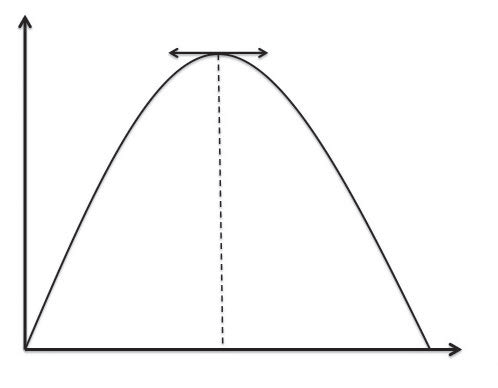
\includegraphics[width=0.75\textwidth]{4º Período/História do Pensamento Econômico/Tradução HPE/Tradução Tópico 9.3/figura 1.png}
    \end{figure}

Os sociólogos construtivistas da ciência reconhecerão na descrição anterior a rigorosa demarcação entre o status comunicacional da curva de Laffer como uma representação visual, de um lado, e as virtudes científicas do embasamento matemático que se pode aplicar a ela, de outro lado, uma curiosa variante do "modelo de difusão" que eles têm criticado ao longo dos últimos 25 anos. Neste modelo, conceitos e ferramentas são inicialmente inventados por gênios cujas reputações vão muito além de seu modesto status como cientistas atuantes. Essas inovações então se difundem para públicos maiores — outros cientistas, estudantes e o público em geral — por meio de um processo que parece automático: as ações de muitos indivíduos e grupos na aceitação e adoção dessas inovações são consideradas garantidas, e as muitas controvérsias que as descobertas geraram inicialmente são geralmente atenuadas e retratadas como ruídos inevitáveis, embora indesejáveis, no processo de difusão. À luz do modelo de difusão, a curva de Laffer é um caso muito estranho porque, pelo menos na descrição dos livros didáticos, sua aceitação parece ter funcionado ao contrário. Em vez de um gênio como os Pasteurs e Diesels do passado, o inventor da curva, Arthur Laffer, frequentemente nem sequer é reconhecido com o título de economista (embora certamente o seja). Os verdadeiros heróis da história são os pesquisadores anônimos trabalhando "a jusante", que forneceram as evidências de que a curva não é empiricamente validada. Mas, estranhamente, apesar do ataque heroico dos autores do livro didático contra a falsidade óbvia da curva de Laffer, a curva ainda está presente no livro, exibida em sua versão canônica e simétrica. Ficamos com uma pergunta que o modelo de difusão não consegue abordar de maneira satisfatória: como ela persistiu?

Talvez um dos modelos alternativos que os sociólogos elaboraram em resposta ao modelo de difusão ofereça uma estrutura melhor para pensar sobre a curva de Laffer. No modelo de "dispersão" — ou "tradução" —, fatos e ferramentas viajam dentro de várias comunidades através do espaço e do tempo. As atitudes que essas diferentes comunidades têm em relação aos objetos que viajam — aceitação, desafio, ignorância ou interesse — diferem muito dependendo de várias contingências. Para serem capazes de viajar, os objetos precisam ser transformados para se adequarem a novos constituintes. Como resultado, sua forma, significado e funcionamento serão afetados, assim como seu status epistemológico. No processo, as atitudes das pessoas que interagem com eles provavelmente evoluirão também (veja Latour 1987, 139–140). Nos últimos anos, vários historiadores da ciência seguiram essa estrutura para construir narrativas mais ricas da disseminação de representações visuais em várias disciplinas. A descrição de David Kaiser (2005) dos diagramas de Feynman na física depende explicitamente do modelo de dispersão, que, em sua opinião, integra duas dimensões importantes dos objetos que estuda: como eles circulam e como persistem. Além disso, historiadores argumentaram que as representações visuais devem ser estudadas na intersecção de dicotomias bem estabelecidas — laboratórios versus museus, artes versus ciências, geometria versus álgebra —, pois é frequentemente no diálogo entre essas que a visualização é discutida (Wise 2006).

O propósito deste capítulo é fornecer um relato histórico da curva de Laffer como um estudo de caso de dispersão. Parece ser um caso ideal para isso porque, como sugeri anteriormente, a trivialidade formal da curva contrasta acentuadamente com a complexidade de sua circulação entre e entre diferentes comunidades: economistas, assessores políticos, propagandistas e jornalistas. Para cada uma dessas comunidades — que, além disso, não eram necessariamente homogêneas dentro de si mesmas —, a curva de Laffer tinha diferentes encarnações e significados; portanto, faz mais sentido usar o plural curvas em vez do singular. No entanto, veremos que a dispersão das curvas de Laffer apresentou duas peculiaridades: primeiro, ao contrário de muitos outros diagramas usados na economia, as instâncias populares da curva de Laffer precederam sua "academização" por economistas profissionais; segundo, apesar das numerosas transformações que a curva sofreu no processo de sua circulação, sua apresentação canônica — a curva simétrica em forma de bala na figura 13.1 — foi reforçada ao longo do tempo. A circulação das curvas de Laffer deve ser explicada pela dinâmica interna de cada uma das comunidades que interagiram com elas, e pelo que acontece na intersecção dessas comunidades, mais importante como consequência da posição ambígua que a profissão econômica manteve em relação ao seu papel na assessoria política. Embora a disciplina sempre tenha estado ansiosa para oferecer conhecimento mais legítimo — do ponto de vista científico — do que o que é circulado em jornais e panfletos, ela também teve que encontrar legitimidade como uma ciência orientada para políticas. Começarei retratando as origens políticas da curva (seção 2); então, passarei para sua subsequente "academização" (seção 3) e generalização (seção 4). Como a discussão a seguir será principalmente histórica em seu conteúdo, discutirei na conclusão algumas implicações para a sociologia do conhecimento e, mais especificamente, para o estudo de práticas representacionais na economia.

\subsubsection{\textbf{O Significado Político da Curva de Laffer Original}}

A curva de Laffer não se originou na literatura acadêmica, e Arthur B. Laffer foi apenas parcialmente responsável por sua circulação. Ela foi, de fato, introduzida por Jude Wanniski em seu livro de 1978 \textit{The Way the World Works}. Nascido em 1936, Wanniski foi contratado como colunista do \textit{Wall Street Journal} em 1972, após anos cobrindo a política energética para vários jornais. Quando seu livro foi lançado, ele acabara de ser forçado a renunciar a essa posição depois que foi descoberto que ele estava distribuindo panfletos para um candidato republicano ao senado. Ele decidiu começar uma carreira como assessor de vários políticos republicanos e criou um negócio para isso, a Polyeconomics. Wanniski era conhecido como um ardente defensor da ``economia de oferta'', um termo que ele havia cunhado em 1976 em contraste com a ênfase do lado da demanda na economia keynesiana sobre a intervenção governamental para estimular o consumo privado e o investimento e reduzir o desemprego. A economia de oferta foi defendida por dois professores de economia, Robert Mundell e Arthur Laffer, que argumentaram que a intervenção estatal tinha efeitos prejudiciais sobre a oferta de bens e mão de obra e era a principal causa da redução do PNB e do aumento do desemprego. Embora Mundell, um ex-estudante de doutorado no MIT que havia lecionado na Universidade de Chicago até 1971, fosse respeitado entre os economistas por seus modelos macroeconômicos internacionais, ele estava se tornando marginalizado na profissão nos anos 1970 após sua produção científica ter diminuído. Laffer, por outro lado, era considerado entre os colegas economistas como um jovem estudioso promissor que havia praticamente cessado o trabalho acadêmico para seguir uma carreira mais politicamente orientada. Depois de estudar em Yale e Stanford e ensinar na escola de negócios de Chicago, ele havia servido como assessor econômico para as administrações Nixon e Ford. De acordo com Wanniski, Laffer havia desenhado a curva que levaria seu nome em um guardanapo de coquetel durante uma reunião com alguns assessores presidenciais em dezembro de 1974.


\begin{figure}[H]
    \centering
    \caption{Gráfico 13.2}
    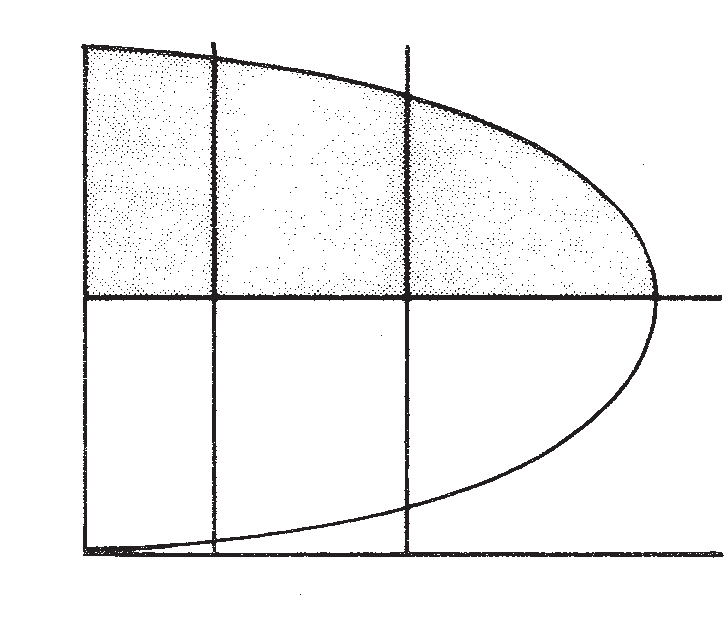
\includegraphics[width=0.75\textwidth]{4º Período/História do Pensamento Econômico/Tradução HPE/Tradução Tópico 9.3/figura 2.png}
    \end{figure}

Na sua representação original, a curva de Laffer apareceu como um diagrama em forma de bala, no qual as receitas fiscais eram representadas no eixo horizontal e a taxa tributária agregada no eixo vertical (figura 13.2). Nas palavras de Wanniski, a curva ilustra a ideia de que ``sempre existem duas taxas tributárias que geram as mesmas receitas'' (Wanniski 1978, 97). Enquanto a parte inferior da curva representa uma relação crescente entre as taxas tributárias e as receitas fiscais, essa relação torna-se decrescente além do ponto E. A interpretação dessa relação é que, quando as taxas tributárias aumentam de zero até qualquer porcentagem abaixo do ponto E, os agentes econômicos pagarão seus impostos mantendo inalterada a sua oferta de trabalho e bens. Nessa faixa inferior, taxas tributárias mais altas gerarão maiores receitas fiscais. No ``intervalo proibitivo'', no entanto, que é a parte além do ponto E, as pessoas decidirão trabalhar menos ou participar de uma economia de escambo (ou negra), o que levará a uma redução da base tributária e subsequente diminuição das receitas fiscais. O ponto E, portanto, aparece como o ponto em que as receitas fiscais seriam máximas. Esse ponto, Wanniski observou, é um ``número variável. É o ponto em que o eleitorado deseja ser tributado... É tarefa do líder político determinar o ponto E e segui-lo em suas variações o mais de perto possível'' (ibid., 98–99, ênfase no original).

Wanniski colocou a curva de Laffer no centro de seu livro de 1978, cuja publicação foi apoiada por Irving Kristol, um ex-colega no \textit{Wall Street Journal} e uma das principais figuras do então emergente movimento neoconservador. A aprovação da Proposição 13 na Califórnia em junho de 1978, que resultou em uma redução drástica das taxas de imposto sobre a propriedade naquele estado, foi seguida por revoltas fiscais em todo o país. Na preparação para as eleições de meio de mandato e a próxima campanha presidencial, havia uma clara percepção entre os republicanos de que era necessário mais do que o discurso conservador tradicional, que defendia um corte nos gastos governamentais e controles sobre preços e salários para estabilizar a inflação. Para esse propósito, a curva de Laffer era oportuna. Ao contrário do discurso direitista ortodoxo da época, que tentava convencer a população de que sacrifícios eram necessários no caminho para o crescimento econômico, a curva de Laffer sugeriu que menos tributação resultaria em mais riqueza para distribuir. Como resultado, economistas do lado da oferta não defendiam um corte no investimento público: ao contrário, um corte de impostos que contribuísse para aumentos nas receitas fiscais permitiria mais gastos governamentais no futuro. Essa foi, em linhas gerais, a ``economia da alegria'' que dominou a campanha de Ronald Reagan a partir de 1978 (Stein 1984).


O livro de Wanniski e a curva de Laffer que ele promoveu forneceram um trampolim para a propaganda do lado da oferta, baseando-se em um populismo antiexperts e na crítica à profissão econômica como um todo. Wanniski argumentou no início de seu livro que os eleitores sabiam mais do que os economistas, no sentido de que seu próprio comportamento poderia contradizer as previsões dos especialistas. Nessa crítica, economistas acadêmicos foram repreendidos junto com conselheiros econômicos por fornecerem teorias irrelevantes e conselhos equivocados. Na visão de Wanniski, a curva de Laffer personificava a falha dos economistas — exceto Mundell e Laffer, claro — em perceber que havia uma fronteira tênue entre uma economia monetária e uma economia de escambo, entre trabalho e não trabalho. O resto do livro tentava demonstrar que a história econômica — desde o declínio do Império Romano até crises econômicas passadas e presentes — poderia ser interpretada usando a curva de Laffer e que as teorias econômicas passadas também poderiam ser encapsuladas usando o arcabouço da curva. No capítulo 8, o autor atacou Keynes e seus principais oponentes, Milton Friedman e os monetaristas da Escola de Chicago. Enquanto a defesa de Keynes pelo gasto deficitário sem cortes de impostos lançaria a economia na faixa proibitiva da curva de Laffer, o apelo de Friedman por um corte nos gastos governamentais resultaria em um aumento nas taxas de juros que, por sua vez, contrabalançaria os efeitos esperados das reduções de impostos. Wanniski argumentou que o que tornava esses dois arcabouços igualmente inválidos era que ambos modelavam a economia em termos de análise de equilíbrio parcial, referindo-se a Alfred Marshall, que analisava um mercado de cada vez. Em contraste, seu próprio modelo, a curva de Laffer, seguiria o arcabouço de equilíbrio geral de Léon Walras, onde todos os efeitos econômicos eram considerados simultaneamente. É por isso que, segundo Wanniski, apenas Laffer e Mundell estavam corretos em sua abordagem, enquanto outros economistas estavam construindo ``edifícios matemáticos elegantes sobre uma fundação de ilusão'' (ibid., 166). Isso constituía nada menos que um insulto à maioria dos economistas mainstream do período pós-guerra, que afirmavam ter revivido a tradição Walrasiana, que, por sinal, era mais, não menos, matemática do que a análise Marshalliana que a maioria havia abandonado.

Diante de tais comentários depreciativos, a maioria dos economistas permaneceu em silêncio. Nenhuma resenha de \textit{The Way the World Works} foi publicada em periódicos acadêmicos de economia, apesar do fato de que tais revistas frequentemente dedicavam espaço à literatura não acadêmica. Admitidamente, alguns economistas expressaram sua desaprovação da curva de Laffer, mas apenas quando escreviam na imprensa popular. Por exemplo, Joseph Minarik foi citado no \textit{New York Times} afirmando que ele havia feito o cálculo e encontrado resultados demasiadamente erráticos para certificar que a curva existia; ``seus projetistas deveriam alisar algumas das rugas antes de oferecê-la ao público'' (Rattner 1978). Até mesmo Laffer recuou um pouco do entusiasmo de Wanniski. Quando questionado por um jornalista para explicar sua curva, ele a apresentou como incorporando dois efeitos conflitantes que as taxas de impostos têm sobre as receitas fiscais: um era o efeito ``aritmético'' ou ``contábil'', que implicava que impostos mais baixos levariam a uma diminuição na receita coletada por dólar de base tributária; e o outro era o ``efeito econômico'', que resultava em uma expansão da base tributária. No entanto, ele não concluiu qual efeito dominaria o outro (citado em Jensen 1978). Em 1979, três dos estudantes de Laffer na Universidade do Sul da Califórnia publicaram um artigo curto no qual tentavam construir uma versão mais elaborada da curva, usando apenas raciocínio diagramático (Canto, Joines e Webb 1979). Neste modelo, a curva foi derivada de um modelo microeconômico uma vez aceito no qual um aumento nas taxas de impostos cria incentivos para se mover do setor de mercado (trabalho) para o setor doméstico (lazer). Este modelo, no entanto, constituiu um sério retrocesso em relação às ambições de Wanniski. Ele ignorou muitas das complexidades em um arcabouço Walrasiano generalizado e baseou sua análise em uma única taxa de imposto imposta sobre a produção do setor de mercado. Além disso, os estudantes realizaram testes empíricos bastante decepcionantes: usando os cortes de impostos de 1962 e 1964 como um experimento, eles tiveram que concluir que era ``quase igualmente provável que os cortes de impostos de Kennedy aumentassem as receitas como que as diminuíssem'' (ibid., 38). Dois artigos subsequentes (Canto, Joines e Laffer 1981; Laffer 1981) tentaram construir modelos mais elaborados de tributação, mas nenhum deles incluiu uma curva de Laffer real. Essas contribuições, que não apareceram em periódicos de economia mainstream, não conseguiram alcançar os economistas acadêmicos. Estes, de fato, consideravam o debate sobre a curva de Laffer como uma distração indesejável do pensamento econômico sério.

\subsubsection{\textbf{A "Academização" da Curva}}

Demorou cerca de três anos até que a curva de Laffer penetrasse na literatura acadêmica. Nesse ínterim, Ronald Reagan se tornou presidente e sua administração já havia tomado medidas para reduzir os impostos. Os economistas da escola de oferta foram bastante influentes nas reformas fiscais. Atuando como consultor do congressista de Nova York, Jack Kemp, Wanniski ajudou a elaborar a proposta de corte de impostos Kemp-Roth de 1978, que serviu de base para a Lei de Recuperação Econômica (ERTA) de 1981. O projeto que foi aprovado pelo Congresso, no entanto, representou um pequeno recuo do plano inicial de Kemp: enquanto Kemp havia aconselhado um corte de impostos de 33\%, aplicado uniformemente a todas as faixas de impostos, a ERTA reduziu as taxas máximas de 70 para 50\% e as taxas mínimas de 14 para 11\%. Embora a reforma tributária não tenha seguido escrupulosamente as prescrições da curva de Laffer, esta ainda era vista como um de seus principais componentes ideológicos na imprensa popular. O aumento das receitas fiscais que os economistas da escola de oferta haviam previsto não ocorreu, e os cortes de impostos resultaram em déficits orçamentários e esforços subsequentes para cortar gastos. Um desses esforços envolveu uma proposta para cortar o financiamento das ciências sociais e comportamentais em 75\%. Escrito por David Stockman, chefe do Escritório de Orçamento e Gestão, ele pressagiava um dano significativo à pesquisa econômica, que dependia fortemente de bolsas da Fundação Nacional de Ciências. O comitê executivo da Associação Econômica Americana, que geralmente evitava questões políticas, expressou preocupações sobre a situação. Seu presidente, William Baumol, escreveu uma carta aos presidentes dos departamentos de economia nos Estados Unidos, incentivando-os a escrever aos membros do Congresso para alertá-los sobre as consequências prejudiciais que tais cortes teriam na busca pelo conhecimento econômico. Em 1981, então, o evangelho dos economistas da escola de oferta estava ameaçando materialmente a comunidade econômica. Como se isso não fosse ruim o suficiente, a saga dos "fracassados" cortes de impostos também estava transformando toda a profissão em motivo de riso aos olhos de outros cientistas e intelectuais, que consideravam a curva de Laffer não apenas um exemplo particularmente fraco de pensamento econômico, mas também um sintoma de que a economia em si era mera ideologia respaldada por matemática medíocre. Característico dessa posição foi a publicação na Scientific American de um artigo de Martin Gardner, um conhecido especialista em matemática recreativa, intitulado "A Curva de Laffer e Outras Risadas na Economia Atual". Zombando do argumento de Wanniski de que o ponto E poderia ser localizado em qualquer lugar ao longo da curva, Gardner introduziu a curva neo-Laffer (figura 13.3). "Como a velha curva de Laffer", escreveu ele, "a nova também é metafórica, embora seja claramente um modelo melhor do mundo real. Como é um reflexo estatístico do comportamento humano, sua forma muda constantemente, como a curva de Phillips, de maneiras imprevisíveis" (Gardner 1981, 27). Gardner não apenas satirizou a curva de Laffer original, mas também zombou de tentativas posteriores de tirar estimativas da curva: "Porque leva muito tempo para reunir dados e ainda mais para analisar todos os parâmetros de mudança, quando uma curva NL é desenhada, ela está desatualizada e não é muito útil" (ibid.).

\begin{figure}[H]
    \centering
    \caption{Gráfico 13.3}
    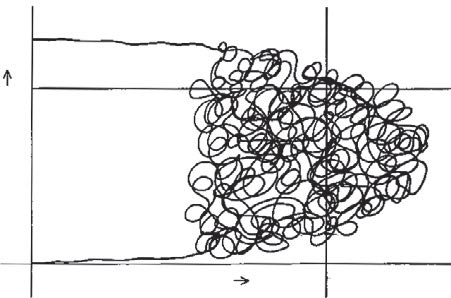
\includegraphics[width=0.75\textwidth]{4º Período/História do Pensamento Econômico/Tradução HPE/Tradução Tópico 9.3/figura 3.png}
    \end{figure}

Enquanto isso, dentro da administração Reagan, havia um crescente descontentamento com a economia da oferta. Entre os conselheiros, monetaristas como Arthur Burns e Alan Greenspan ainda acreditavam que o controle da oferta monetária por meio do aumento das taxas de juros deveria prevalecer sobre os cortes de impostos como forma de garantir o crescimento econômico a longo prazo. O monetarismo, de fato, era o principal princípio que havia orientado as ações do Federal Reserve desde 1979, quando Paul Volcker foi nomeado presidente. Em contraste, os verdadeiros crentes na economia da oferta estimaram que a política monetária atual havia impedido que os cortes de impostos rendessem as receitas esperadas. À medida que as tensões aumentavam, o debate político se tornava desagradável. Wanniski, por exemplo, escreveu em julho de 1981: “Milton Friedman não é um homem grande, mas é muito pesado. Suas ideias econômicas monetaristas... estão prejudicando o velho amigo do laureado com o Nobel, Ronald Reagan, a economia dos Estados Unidos e, indiretamente, todos os nossos parceiros comerciais. O professor Friedman tem pouco mais de um metro e meio de altura, mas sua sombra se estende pela última década de inflação global” (Wanniski, 1981). Em reação a tanta acrimônia, muitos economistas sentiram que era hora de uma investigação acadêmica mais séria sobre a curva de Laffer, que não apenas levaria o debate em uma direção mais rigorosa, mas também restauraria a credibilidade da profissão econômica. A resposta dos economistas, naturalmente, implicava no aumento da matematização dos modelos concorrentes. Duas contribuições, publicadas em 1982, provaram ser particularmente influentes em trazer a curva de Laffer para o debate acadêmico.

Primeiro, Don Fullerton (1982) ofereceu um modelo analítico completo da curva que a tornaria uma hipótese testável. Ele observou que, enquanto a típica curva de Laffer representa como as receitas fiscais variam com as mudanças nas taxas de impostos, o fator-chave para determinar se estamos na faixa normal ou proibitiva é a elasticidade da oferta do fator: o grau em que uma variação no imposto afetará a oferta do fator - trabalho ou capital - sendo tributado. Como resultado, uma infinidade de curvas de Laffer pode ser imaginada - com uma curva para cada valor de um dado fator de oferta elástica. Fullerton, portanto, postulou que a curva de Laffer não era uma "colina", como a representação canônica mostrava, mas uma "cordilheira", já que tinha que ser representada em um diagrama tridimensional com a elasticidade da oferta do fator como a terceira dimensão. Fullerton só desenhou o "cume" da cordilheira, que mostrava uma relação descendente entre as taxas de impostos e a elasticidade da oferta do fator, representando cada ponto ao longo da curva onde as receitas fiscais seriam máximas (veja a figura 13.4). A faixa normal está localizada abaixo da curva, enquanto a área acima da curva corresponde à faixa proibitiva. Usando um modelo econométrico de equilíbrio geral dos Estados Unidos, Fullerton tentou estimar a nova curva e eventualmente a forma das curvas de Laffer para várias taxas de impostos e elasticidades de oferta de fatores. Ele concluiu que, em teoria, os EUA poderiam estar operando na faixa proibitiva no caso em que os salários são tributados a uma taxa muito alta. No entanto, levando em conta as estimativas econométricas anteriores das elasticidades da oferta de trabalho para vários grupos da população, ele mostrou que, sob suposições realistas, a taxa de imposto proibitiva teria que ser bem acima da taxa atual nos EUA. Em outras palavras, a curva de Laffer começaria a diminuir a uma taxa de imposto muito mais alta do que as representações anteriores sugeriam.

\begin{figure}[H]
    \centering
    \caption{Gráfico 13.4}
    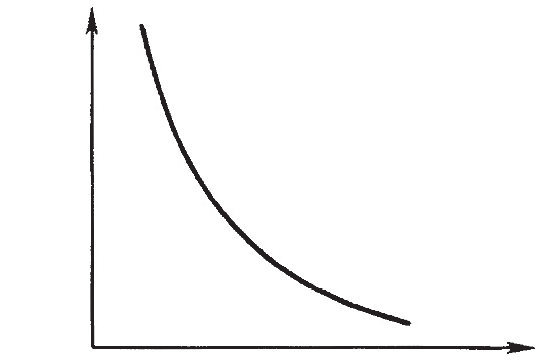
\includegraphics[width=0.75\textwidth]{4º Período/História do Pensamento Econômico/Tradução HPE/Tradução Tópico 9.3/figura 4.png}
    \end{figure}

O breve artigo de James Buchanan e Dwight Lee (1982) constituiu uma abordagem completamente diferente para a curva de Laffer. Os autores não tentaram questionar suas fundações, mas sim suas consequências dentro do arcabouço econômico da teoria da escolha pública. Ao contrário da maioria dos economistas, que presumiam que o Estado era um observador externo operando em favor de resultados socialmente desejados, os teóricos da escolha pública argumentavam que o governo consistia em agentes econômicos que maximizavam a utilidade e agiam em benefício próprio. A partir deste ponto de partida, Buchanan e Lee procuraram explicar como um governo supostamente racional acabaria escolhendo uma taxa de imposto menos do que ótima. Sua resposta consistiu em argumentar que a curva de Laffer que outros haviam tentado avaliar até agora era, na verdade, a representação de uma relação que só ocorreria a longo prazo, enquanto o governo estava mais propenso a agir de acordo com objetivos de curto prazo. Em sua estrutura, a diferença entre os efeitos de curto e longo prazo é o tempo que leva para os contribuintes se ajustarem às mudanças na tributação. Visualmente, sua representação (figura 13.5) consiste em uma curva de Laffer de longo prazo (LRLC) e várias curvas de Laffer de curto prazo (SRLC). Para cada ponto localizado na LRLC, existe uma SRLC diferente que é mais favorável ao governo. Isso significa que, como os contribuintes não ajustam totalmente seu comportamento à taxa de imposto existente no curto prazo, é sempre melhor para o governo aumentar sua taxa de imposto acima do nível que renderia receitas máximas a longo prazo. No entanto, o governo tem que escolher uma taxa de imposto localizada na LRLC porque é a única maneira de garantir uma base tributária. Se a taxa de imposto estivesse localizada além da curva, não haveria renda para tributar. Eventualmente, a taxa de imposto escolhida será aquela que renderá receitas máximas em uma SRLC e que está simultaneamente localizada em algum lugar na porção decrescente da LRLC. Esta situação, argumentam Buchanan e Lee, é estável porque não há incentivo para o governo reduzir seus impostos no curto prazo, que é o único horizonte de planejamento com o qual se preocupa. Portanto, a situação não ótima vai persistir ao longo do tempo. A contribuição de Buchanan e Lee foi particularmente impressionante: ao contrário das tentativas anteriores de aprofundar as implicações analíticas da curva de Laffer, sua versão desta envolveu nenhum outro formalismo matemático além de sua representação diagramática. A razão para isso é que os autores, ao contrário de Fullerton (1982), não estavam interessados em questionar a forma da curva de acordo com dados do mundo real. Em vez disso, eles se concentraram na mera possibilidade de que a curva exista. Ao fazer isso, eles puderam abordar uma questão de teoria política: como governos racionais acabam agindo contra seus próprios interesses? Nesse sentido, a curva de Laffer apareceu não como um modelo que precisa de refinamento, mas como um motor de descoberta.

    \begin{figure}[H]
    \centering
    \caption{Gráfico 13.5}
    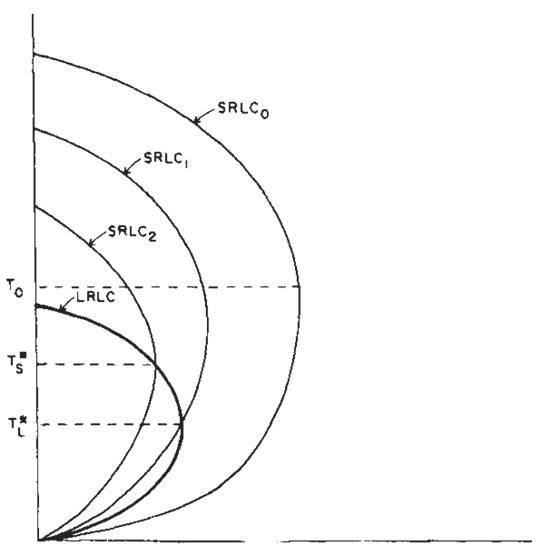
\includegraphics[width=0.75\textwidth]{4º Período/História do Pensamento Econômico/Tradução HPE/Tradução Tópico 9.3/figura 5.png}
    \end{figure}

Embora tenham levado a curva de Laffer em duas direções diferentes, as respectivas contribuições de Fullerton e Buchanan e Lee participaram de sua legitimação como uma ferramenta acadêmica, fornecendo um ponto de partida respeitável para pesquisas futuras.

\subsubsection{\textbf{A Generalização das Curvas de Laffer}}

É impressionante que justamente no momento em que a curva de Laffer foi atacada como um projeto político, ela começou a atrair cada vez mais atenção dos economistas acadêmicos. Em 1986, embora novos cortes de impostos estivessem sendo preparados, a curva de Laffer havia praticamente desaparecido do debate público. Em 1984, Herbert Stein, ex-conselheiro econômico de Nixon, resumiu o sentimento geral: "Entre 1981 e 1983, o país passou de um entusiasmo efervescente pela redução de impostos para um triste reconhecimento de que os impostos eram muito baixos - que somos... uma sociedade subtributada" (Stein 1984, 356). No livro de Stein, a curva de Laffer foi representada como uma curva em forma de sino acentuadamente assimétrica, com a mudança da faixa normal para a faixa proibitiva ocorrendo aproximadamente a uma taxa de imposto de 80\%. Stein observou: "A imagem convencional na qual a curva é simétrica e atinge seu ponto alto a 50\% tem apenas uma justificativa estética" (ibid., 247). No entanto, a mesma curva de Laffer simétrica foi posteriormente dispersa pela literatura científica ao longo de três diferentes linhas de desenvolvimento: primeiro, como base para hipóteses econométricas adicionais; segundo, para explorações mais profundas de sua análise subjacente; e finalmente, para aplicações além das finanças públicas.

Na primeira linha, para o desenvolvimento de hipóteses testáveis, a curva de Laffer não assumiu muita importância. Na verdade, a dificuldade em fazer estimativas empíricas a partir dela era que havia muitas variáveis que tinham que ser simplificadas ou ignoradas: mudanças na distribuição de renda, a complexidade das estruturas tributárias, a forma como as receitas fiscais eram redistribuídas entre os contribuintes, etc. Consequentemente, as estimativas empíricas do pico variavam de um estudo para outro, cobrindo uma faixa entre 40 e 90\%. Além disso, o modelo da curva de Laffer não fornecia uma base clara para comparar tais estimativas entre si. Uma solução foi passar de testar a curva de Laffer para tratar as consequências da vida real de cortes de impostos específicos como descobertas experimentais. Foi isso que Austan Goolsbee, economista da Universidade de Chicago, fez em 1999. Estudando várias mudanças de impostos na história dos EUA, Goolsbee argumentou que nenhum efeito particular sobre as receitas poderia ser identificado que informaria a política. Ele concluiu que "[a] noção de que os governos poderiam arrecadar mais dinheiro cortando as taxas é, de fato, uma ideia gloriosa... Infelizmente para todos nós, os dados do registro histórico sugerem que é improvável que seja verdade em algo como as taxas marginais de impostos de hoje" (Goolsbee 1999, 44). O que é interessante aqui para o nosso propósito é que Goolsbee, embora tenha se referido à curva de Laffer em todo o seu artigo, na verdade não testou a curva, mas apenas a ideia de que taxas marginais de impostos mais altas podem reduzir as receitas do governo. O alvo de Goolsbee, na verdade, era Martin Feldstein, um economista com credenciais acadêmicas mais sólidas do que Laffer. Feldstein havia fornecido justificativas teóricas para a redução de impostos já no meio da década de 1970 e havia se envolvido na reforma tributária durante o segundo mandato de Reagan, precisamente quando os economistas da oferta haviam perdido sua influência no governo. Goolsbee (1999, 9) distinguiu o trabalho acadêmico de Feldstein da "curva de Laffer convencional", que ele disse "não existe". Ele não citou nenhum artigo de Laffer, não reproduziu a famosa curva em lugar algum de seu artigo, e não fez nenhuma referência à versão, até então, quase universalmente ridicularizada que Wanniski e outros economistas da oferta haviam oferecido no final da década de 1970. Em uma seção de discussão e comentário publicada com o artigo, Robert E. Hall começou observando que Laffer não deveria ter sido mencionado no título de forma alguma (em Goolsbee 1999, 48). No entanto, o que o artigo de Goolsbee sinalizou foi que, no final da década de 1990, o termo "curva de Laffer" havia se desvinculado um pouco de suas origens para servir como uma marca registrada para o argumento academicamente respeitável de que cortes de impostos, ao aumentar a oferta de trabalho, ajudariam a aumentar tanto as receitas nacionais quanto governamentais.

O segundo tipo de estudo acadêmico tentou explorar as complexidades analíticas mais profundas da curva de Laffer. Em vez de tentar estimar onde o pico da curva ocorreria, esses estudos mostraram um interesse crescente na questão de se um ponto de mudança ocorre, e portanto questionaram a forma da própria curva. Malcomson (1986), por exemplo, estudou a possibilidade de que a curva inclinasse para cima para todas as taxas médias de impostos. Essa discussão foi perseguida nas páginas do Journal of Public Economics entre 1986 e 1991. Gahvari (1989) provou que no arcabouço de Malcomson, uma condição suficiente para a curva ter uma parte descendente é que a receita tributária seja redistribuída aos contribuintes na forma de uma soma fixa. Guesnerie e Jerison (1991) tentaram generalizar a curva de Laffer sugerindo que ela poderia ser substituída por uma infinidade de curvas correspondentes a várias funções de receita tributária em um arcabouço de equilíbrio geral. Embora seu artigo dissesse que era impossível tirar conclusões de política, porque era impossível prever se uma diminuição nas taxas de impostos resultaria em maiores receitas fiscais, sua principal contribuição foi ampliar a relevância da curva de Laffer. Enquanto no modelo original de Laffer o foco havia sido exclusivamente nas receitas fiscais, Guesnerie e Jerison argumentaram que um arcabouço de equilíbrio geral deveria se concentrar no bem-estar social também. Como as receitas fiscais são usadas para financiar bens públicos, taxas de impostos mais altas resultarão em dois efeitos conflitantes: primeiro, taxas mais altas aumentarão o bem-estar social, porque as pessoas se beneficiarão dos bens públicos adicionais; mas, em segundo lugar, o aumento resultante nos preços dos bens privados terá um efeito prejudicial ao bem-estar social. Isso leva a múltiplos equilíbrios possíveis que renderiam receitas fiscais máximas, mas será praticamente impossível saber quais taxas realmente maximizariam o bem-estar social. Ao buscar generalização e rigor analítico, esses modelos dependem de formalismos cada vez mais complexos. Embora indubitavelmente tenham demonstrado que a versão didática da curva de Laffer era um caso especial de uma relação mais geral com pouca chance de ocorrer na vida real, eles também ajudaram a substanciar a afirmação de que a curva poderia existir em teoria. Em consequência, no final da década de 1990 era muito provável que se deparasse com curvas de Laffer padrão na literatura mainstream.

Um terceiro aspecto do uso da curva de Laffer na literatura econômica recente foi derivado do modelo Buchanan-Lee de 1982, que ofereceu o arcabouço mais facilmente transponível para estudar casos práticos. Um exemplo significativo é um artigo de Clark e Lee (1996), que invoca a curva de Laffer em um estudo sobre política de sentença criminal. Seu artigo traçou a "curva de Laffer de sentença" para cada comprimento médio de sentença que exigia espaço prisional (figura 13.6). De acordo com seu modelo, uma redução no comprimento médio da sentença, que normalmente deveria reduzir a necessidade de espaço prisional, poderia levar ao efeito oposto, à medida que as taxas de criminalidade aumentam em resposta a maiores incentivos para violar a lei. Usando uma análise bastante semelhante à de Buchanan e Lee (1982), Clark e Lee mostraram que o governo provavelmente escolheria um comprimento médio de sentença ineficientemente baixo que não minimizaria a necessidade de espaço prisional. Como no modelo Buchanan-Lee, essa situação subótima pode persistir, porque a curto prazo o governo não teria interesse em estender os comprimentos das sentenças.

\begin{figure}[H]
    \centering
    \caption{Gráfico 13.6}
    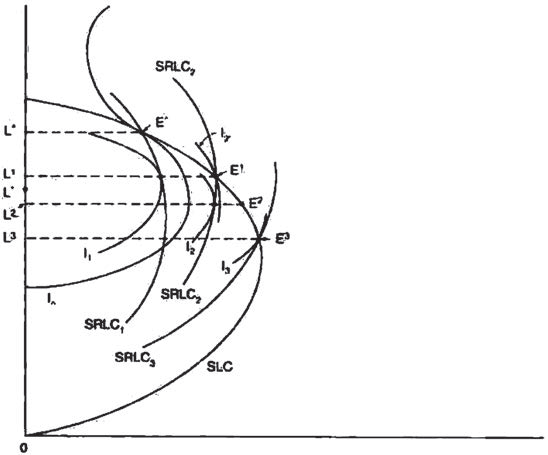
\includegraphics[width=0.75\textwidth]{4º Período/História do Pensamento Econômico/Tradução HPE/Tradução Tópico 9.3/figura 6.png}
\end{figure}

Shmanske (2002) forneceu outra aplicação do arcabouço de Buchanan-Lee, desta vez em um estudo sobre a economia da educação. O ponto de partida de Shmanske era a noção de que algumas escolas poderiam aliviar a carga de seu currículo na expectativa de que isso alcançaria um nível mais alto de matrículas. No entanto, além de um certo ponto, eles acabariam com matrículas insuficientes por causa da degradação da reputação da escola. Além disso, tal degradação impediria a escola de endurecer seu currículo no futuro, porque não seria suficientemente crível para fazê-lo. Tais aplicações metafóricas da curva de Laffer além do domínio das finanças públicas começaram a aparecer em publicações acadêmicas em meados da década de 1990. Na imprensa popular, também houve indicações de tal uso metafórico desde o final da década de 1980. No New York Times, o político democrata Ed Markey (1988) se referiu a uma "versão termonuclear da curva de Laffer", que ele explicou como a noção paradoxal de que "[s]ob Reagatomics, agora construímos mais armas nucleares e melhoramos nossas capacidades de primeiro ataque para ter menos armas nucleares e reduzir a ameaça de um primeiro ataque nuclear desarmante." O uso da curva fora dos limites tradicionais da economia parecia atender a uma demanda social maior por modelos econômicos simples com implicações práticas para situações da vida real. Nesse contexto, a curva de Laffer se tornou uma metáfora difundida para explicar os erros de um governo supostamente racional.

\subsubsection{\textbf{Conclusão}}
John Maynard Keynes certa vez observou que os diagramas em economia compõem parte daquele "aparato elegante que geralmente exerce uma atração poderosa sobre os iniciantes inteligentes, que todos nós usamos como inspirador e um controle sobre nossas intuições e como um registro resumido de nossos resultados, mas que geralmente cai no esquecimento à medida que penetramos mais profundamente nos recessos do assunto" (Keynes 1924, 332 – 333). Relembrando a história da curva de Laffer, podemos concordar parcialmente com a observação de Keynes: a curva de Laffer exerceu fascínio sobre os "iniciantes inteligentes" — neste caso, principalmente não economistas — e serviu como um "inspirador" para modelos econômicos mais elaborados. No entanto, é mais difícil afirmar que a curva original caiu no esquecimento à medida que os modelos se tornaram cada vez mais técnicos, porque sua representação canônica parece ter sido reforçada no processo. Enquanto a narrativa anterior explicou como isso aconteceu nos últimos 30 anos, é hora de refletir sobre as razões para a circulação persistente da curva. Duas linhas de interpretação podem ser apresentadas, uma baseada no status da curva de Laffer como uma representação visual localizada na interseção entre pesquisa e política, e a outra envolvendo o contexto institucional específico que envolve sua circulação.

Esta breve história da curva de Laffer mostra que ela foi inicialmente concebida como uma representação simples de uma realidade que se supunha ser complexa: uma realidade que envolvia uma estrutura tributária complicada e tantos comportamentos diferentes quanto os contribuintes individuais poderiam adotar em resposta às mudanças nas taxas de impostos, sem mencionar os efeitos cumulativos que tais comportamentos poderiam gerar no nível macroeconômico. No entanto, os economistas não estavam em posição de criticar a pretensão de uma curva simples de retratar tais relações intrincadas, porque no passado recente eles haviam usado várias curvas igualmente simples para retratar o funcionamento da economia como um todo. Por que tais representações visuais simples são tão persistentes? A resposta é que enquanto a matematização subsequente de tais curvas simples pode aumentar sua credibilidade aos olhos dos pesquisadores mais teoricamente inclinados, também as torna cada vez menos atraentes para a política pública. No caso da curva de Laffer, sua simplicidade ajuda a explicar por que as versões mais matematicamente sofisticadas da curva não circularam amplamente, mesmo entre os economistas. Portanto, uma conclusão geral que pode ser tirada desta narrativa é que as representações econômicas que reivindicam forte relevância política e, consequentemente, atravessam a fronteira entre a pesquisa acadêmica e a política, provavelmente persistirão ao longo do tempo, apesar de, e talvez até por causa de, sua falha em resistir ao processo de refinamento técnico.

Ainda assim, a academização da curva de Laffer também deve ser entendida à luz do contexto sociológico e institucional mais amplo ao longo do último século que moldou o papel dos economistas na formulação de políticas nos Estados Unidos. Fourcade (2009) argumentou que o que era específico sobre a economia americana era seu enraizamento acadêmico, em contraste com o tipo mais burocrático de expertise econômica que prevalecia na Europa continental. A partir da década de 1930, na ausência de uma elite tecnocrática preexistente, os governos americanos passaram a depender cada vez mais de economistas acadêmicos para realizar várias tarefas técnicas. A legitimidade dos economistas como especialistas em políticas dependia das expectativas de seus sólidos padrões acadêmicos, mas também de sua capacidade de penetrar no mercado e vender suas habilidades por meio de organizações públicas e privadas sem fins lucrativos que não tinham agendas políticas definidas, como a Ford Foundation ou a Brookings Institution. Daí a relação dos economistas com a política era muitas vezes indireta e ambígua. A dispersão da(s) curva(s) de Laffer ocorreu na última parte do século XX, quando esse modelo de expertise econômica enfrentou uma crise, à medida que um novo tipo de think tank crudamente ideológico tentava competir com os economistas acadêmicos no mercado de expertise técnica. Quando alguns desses think tanks, como o Cato Institute com o qual Laffer e seus aliados estavam envolvidos, começaram a influenciar a política, a relação dos economistas com a política tornou-se ainda mais ambígua. Enquanto alguns economistas academicamente respeitáveis estavam interessados nesta nova oportunidade de disseminar suas ideias, outros estimaram que deveriam elevar ainda mais os padrões científicos de sua disciplina para fornecer um baluarte contra o que consideravam uma ameaça à sua legitimidade. Essas atitudes conflitantes podem explicar o desprezo que prevaleceu entre os economistas acadêmicos na recepção inicial da curva de Laffer, bem como sua posterior apropriação como um objeto de pesquisa aceitável. Enquanto, nas últimas duas décadas ou mais, os sociólogos da ciência procuraram mostrar que o estudo das representações na prática científica deve prestar atenção aos contextos sociais nos quais essas representações são produzidas, a história da curva de Laffer mostra que, para representações particulares, a noção de contexto teria que ser estendida para incluir os aspectos culturais, sociais e institucionais mais amplos que enquadram e legitimam o discurso científico.

\subsubsection{\textbf{Agradecimentos}}

Gostaria de agradecer a Béatrice Cherrier e José Edwards por me ajudarem a localizar alguns dos primeiros artigos sobre a curva de Laffer, Roger Middleton por compartilhar rascunhos não publicados e Fabian Gouret por comentários úteis. Além disso, me beneficiei de observações perspicazes, correções e referências adicionais fornecidas por três árbitros anônimos e pelos editores deste volume. As ressalvas habituais se aplicam.


\end{document}


